
\section{Dielectric slab} % references to ->%{{{
%% TODO co znamená  " {\infty}-P  KP   KP-DM  " ??
The structure composed of alternating dielectric layers, effectively a one-dimensional photonic crystal, has been investigated thoroughly in the previous decades. We review it mostly for comparison with the structures presented in the following. 

\begin{figure}[ht] \caption{Dispersion curves for an one-dimensional photonic crystal, computed using PWEM. The side plots show the shape of the fields in the $(y,z)$ plane, at the frequencies of the band edges. Note that each field plot spans two unit cells. The electric field $E_x$ is plot as color map. \textbf{a)} In free space, \textbf{b)} in dielectric layers with permittivity $\varepsilon = 12$ and 15 \% thickness (outlined by black lines)} \label{fg_1dbd} \centering 
\textbf{a)}	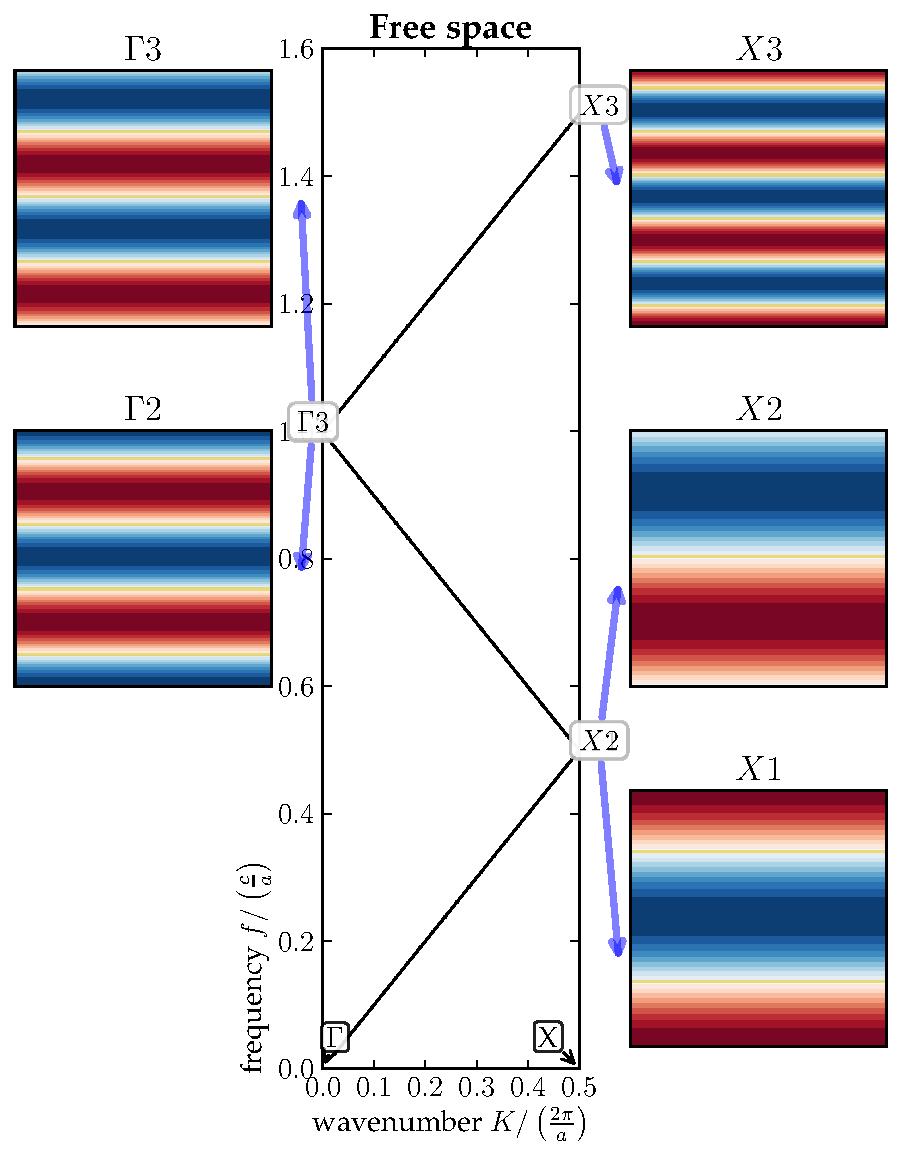
\includegraphics[width=8cm]{img/Slab_eps001_PWEM.pdf}
\textbf{b)}	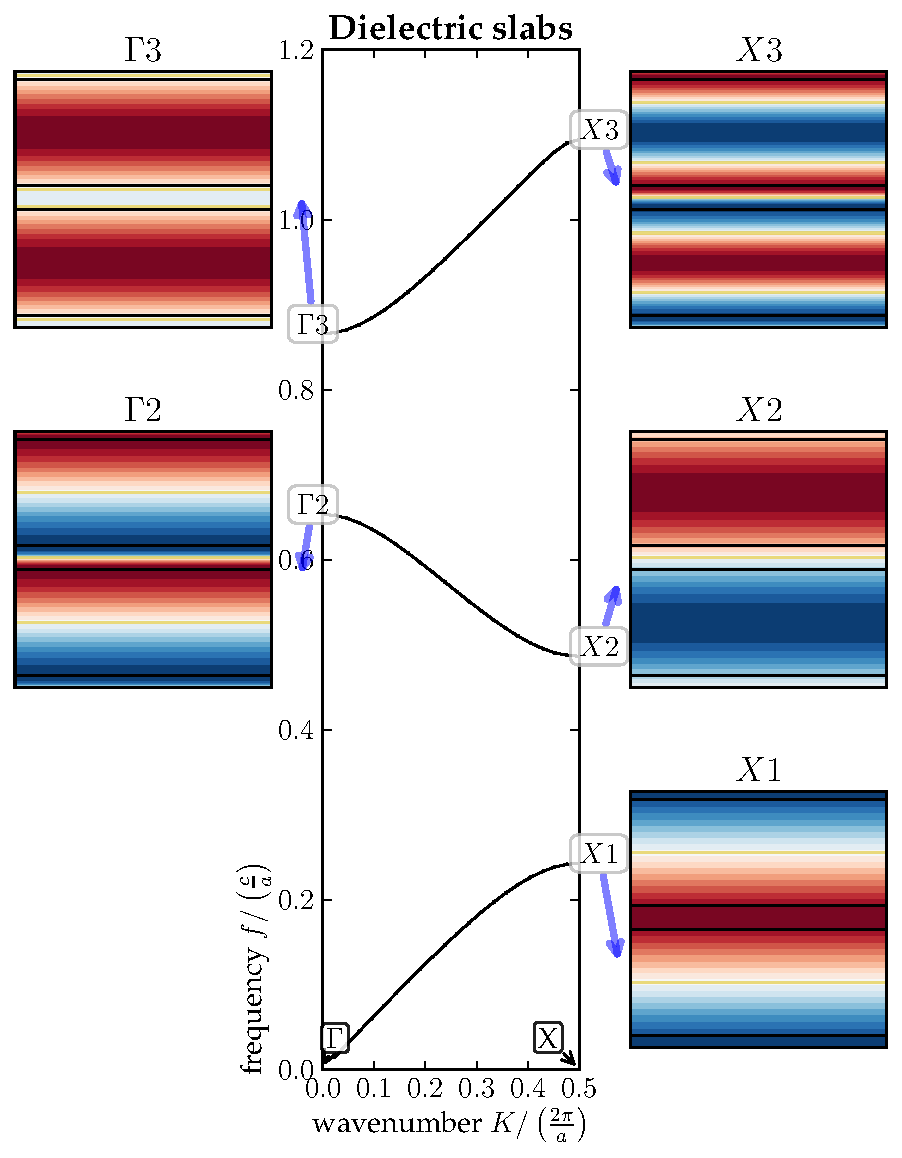
\includegraphics[width=8cm]{img/Slab_eps012_d15.pdf}
\end{figure}
% TODO draw and append axes+colorbar to the field distribution plots
% TODO visualise the permittivity, but how?

In Fig. \ref{fg_1dbd}a, we can see the folded dispersion curves for a plane wave propagating in vacuum, as already discussed above. 
%As predicted by the Bloch-Floquet theorem (\ref{eq_bloch}), the fields are periodic over each cell whenever the wavenumber $k$ touches the Brillouin zone boundary. 
To save space, we plot the  dispersion curves as \textit{folded}, but one can easily imagine how the curve unfolds into a straight light line. For any frequency $f$, there is a wavenumber $k$ corresponding to a propagating wave. 


The situation is different when we introduce periodic dielectric layers as in Fig. \ref{fg_1dbd}b. In the band structure, we observe allowed bands with \textit{band gaps} between them. At the frequencies in a bandgap, the wave can not propagate through the structure. The first photonic band ends when half the wavelength matches the cell spacing, i.e. when $2\pi / K= a/2$. The next band starts at the same wavenumber $K$, but the wave now has higher frequency because it is shifted by half its period so that it maximizes electric energy in air. For a 1-D photonic crystal, we can generally conclude that in order to move up on the frequency axis,
\begin{enumerate}
 \item{within each photonic band, one nodal plane per unit cell is added\footnote{In this paper, the mode plots show $2\times 2$ unit cells for clarity.},} 
 \item{within each photonic band gap, the wave shifts the most of electric field energy into lower-permittivity medium\footnote{Note that the band gaps do not have the same width on the frequency scale. For a certain thickness of the high-dielectric layer that corresponds to the Fabry-Pérot resonance, no frequency difference at all results from shifting the wave. In this case the band gap attains zero thickness, as is illustrated in Fig. \ref{fg_ebar_radiusscan}a for $r\approx20\,\upmu$m and $f\approx1.6$ THz. In other words, there may be a \textit{gap-less} transition between photonic bands.}, while the number of nodal planes remains constant. }
 \end{enumerate}

Such a shifting between waves at the lower and upper boundaries of the band gap is typical of classical \textit{Bragg} gaps that are responsible for the dispersion of the 1-D photonic crystal. 

\begin{figure} \caption{img/Slab\_eps001\_PWEM.pdf}  \centering 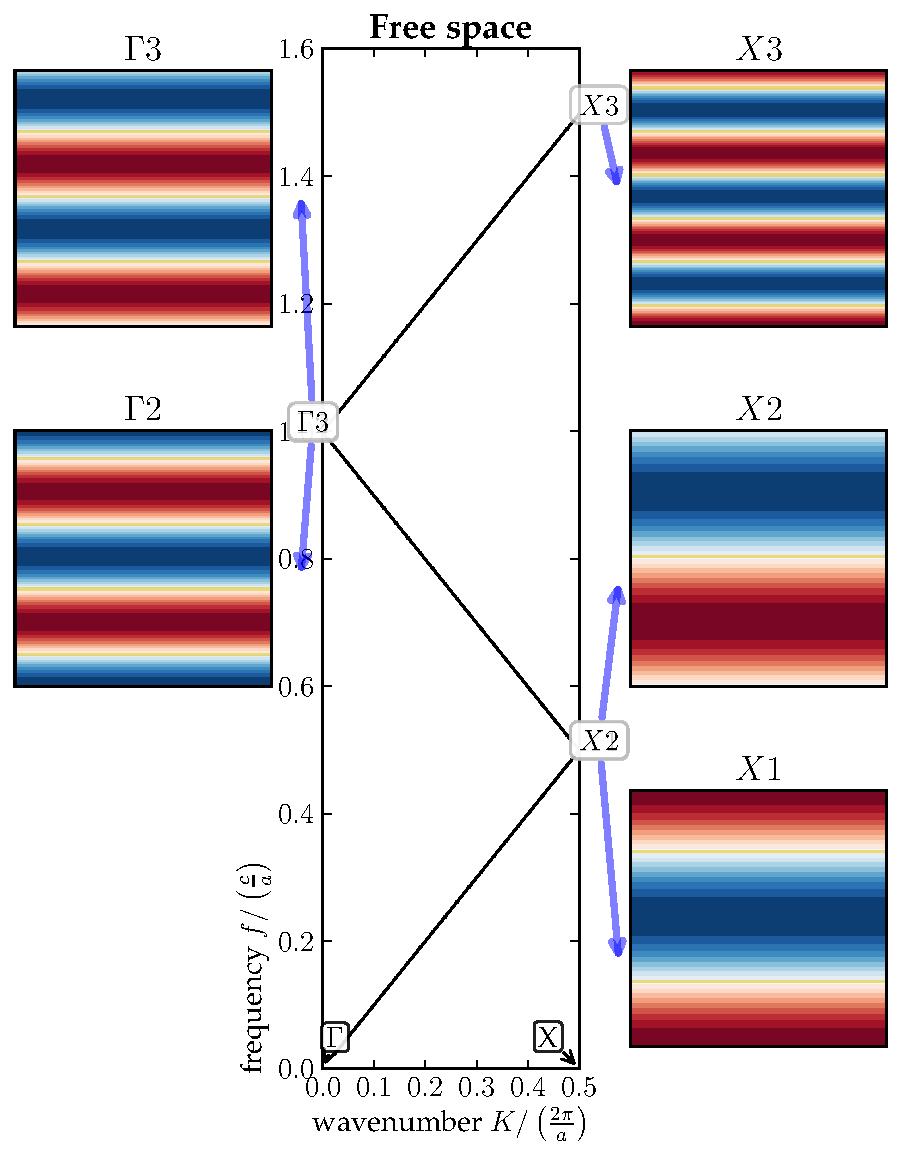
\includegraphics[width=10cm]{img/Slab_eps001_PWEM.pdf} \end{figure} \clearpage
\begin{figure} \caption{img/Slab\_eps012\_d15.pdf}  \centering 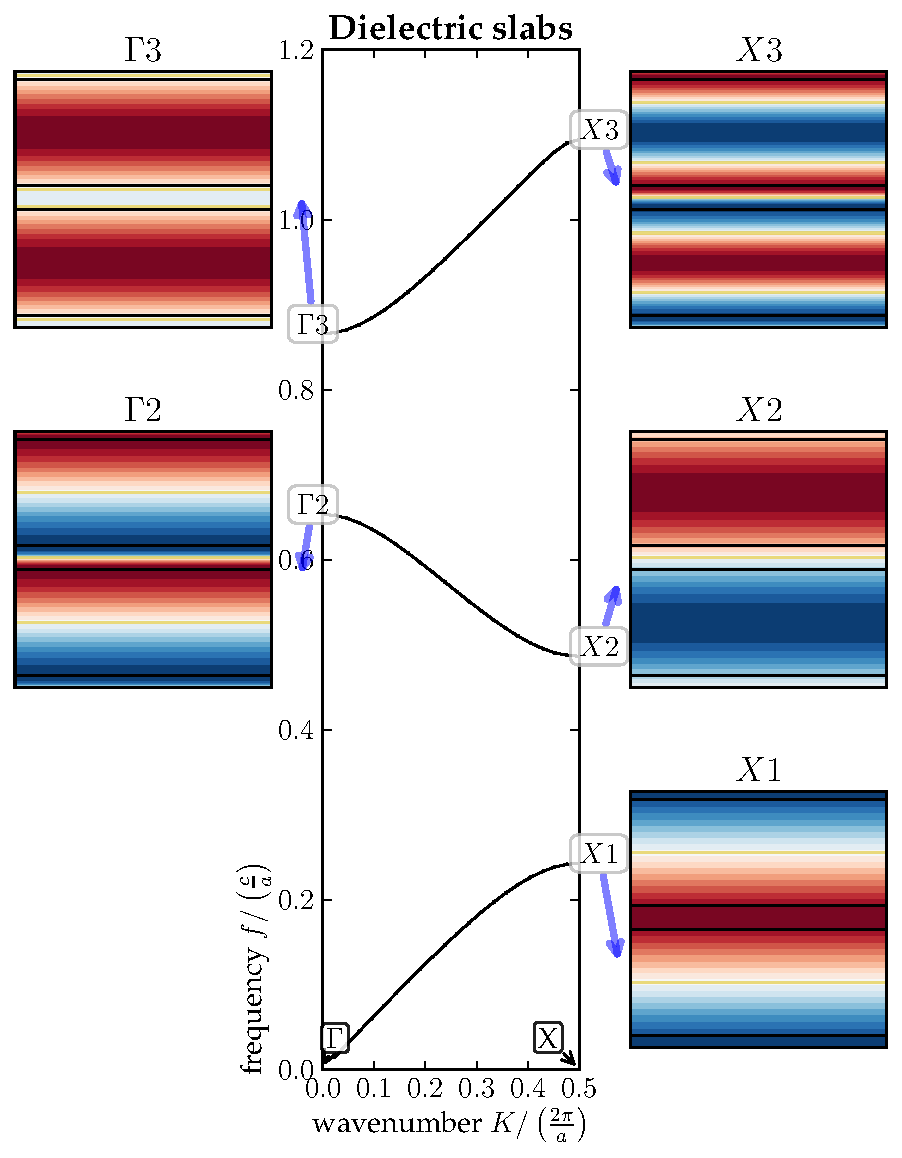
\includegraphics[width=10cm]{img/Slab_eps012_d15.pdf} \end{figure} \clearpage
%}}}

\subsection{Finite planar structure with defect mode} % references to ->
A defect-mode transmission peak of 1.5\% energy transmission appears in the band gap.
It can be tuned from 173 to 184 GHz by application of electric field (40 kV/cm) to the defect STO layer \cite{skoromets2013}.
%}}}

\section{Wire medium} % references to -> %{{{
\add{
We assume the medium is inductive $\quad \Rightarrow \quad  \varepsilon(f) = 1 - \frac{f_p^2}{f^2}$. 

\begin{itemize} \item{What is the plasma frequency $f_p$ for wires (with radius $r$ and spacing $a$)?} \end{itemize}

Pendry \textit{et al.} 1996: $\sqrt{\frac{c^2}{2\pi \, a^2 \, \log(\frac{a}{r})}}$

Maslovski \textit{et al.} 2003: $\sqrt{\frac{c^2}{2\pi \, a^2 \, \log\left(\frac{a^2}{4r (a-r)}\right)}}$

\begin{itemize} \item{How these models compare to the simulation?} \end{itemize}

CITE J. B. Pendry, A. J. Holden, W. J. Stewart, and I. Youngs, \textit{"Extremely low frequency plasmons in metallic meso structures,"} phys. rev. lett., vol. 76, pp. 4773–4776, 1996.  \\
CITE Maslovski, S. I., Tretyakov, S. A. and Belov, P. A. (2002), \textit{Wire media with negative effective permittivity: A quasi-static model.} Microw. Opt. Technol. Lett., 35: 47–51. doi: 10.1002/mop.10512

}


\begin{figure} \caption{img/XCylWire\_a100r4.pdf}  \centering 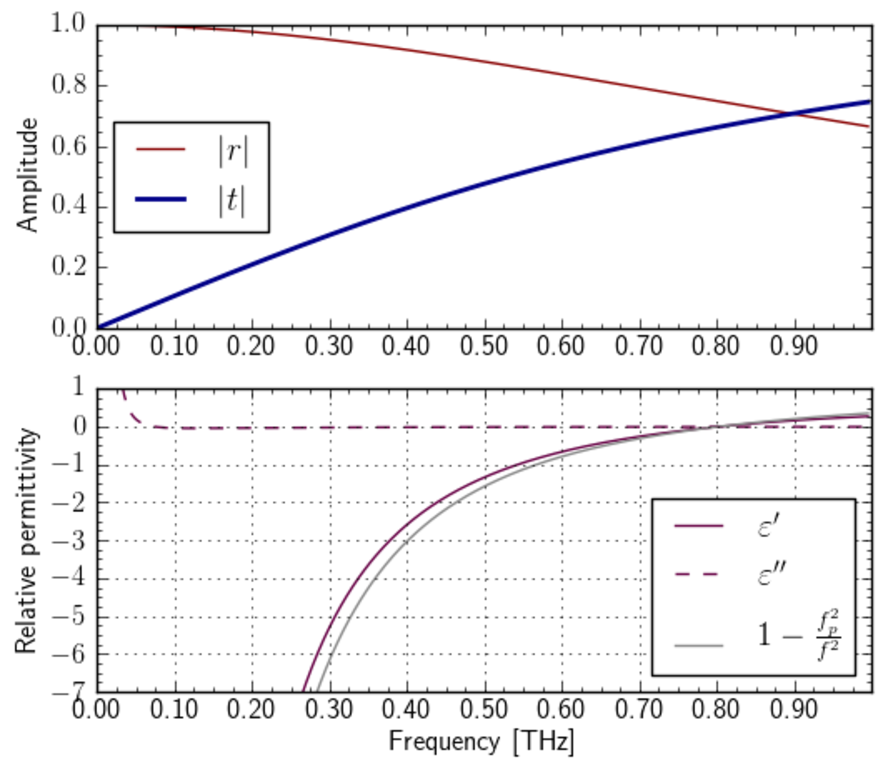
\includegraphics[width=10cm]{img/XCylWire_a100r4.pdf} \end{figure} \clearpage
\begin{figure} \caption{img/EWire\_plasmaF\_radiusscan.pdf}  \centering 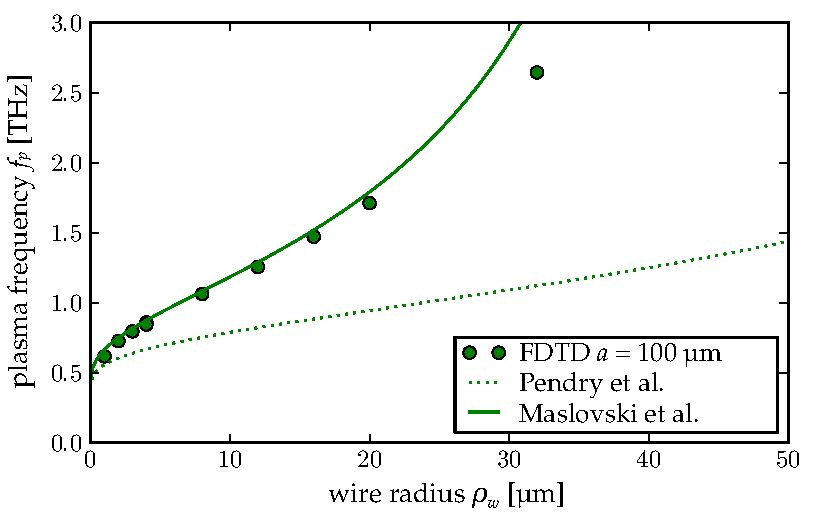
\includegraphics[width=10cm]{img/EWire_plasmaF_radiusscan.pdf} \end{figure} \clearpage
\begin{figure} \caption{img/EWire\_plasmaF\_spacingscan.pdf}  \centering 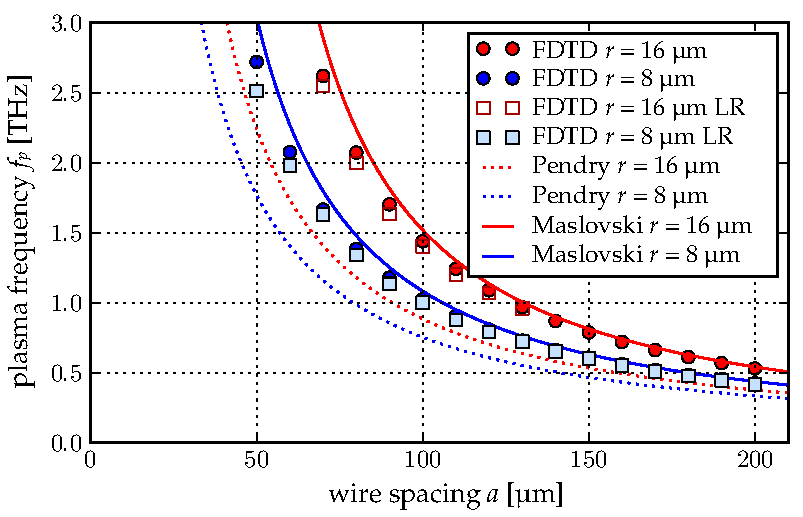
\includegraphics[width=10cm]{img/EWire_plasmaF_spacingscan.pdf} \end{figure} \clearpage
\begin{figure} \caption{img/EWire\_r03\_FDTDwide.pdf}  \centering 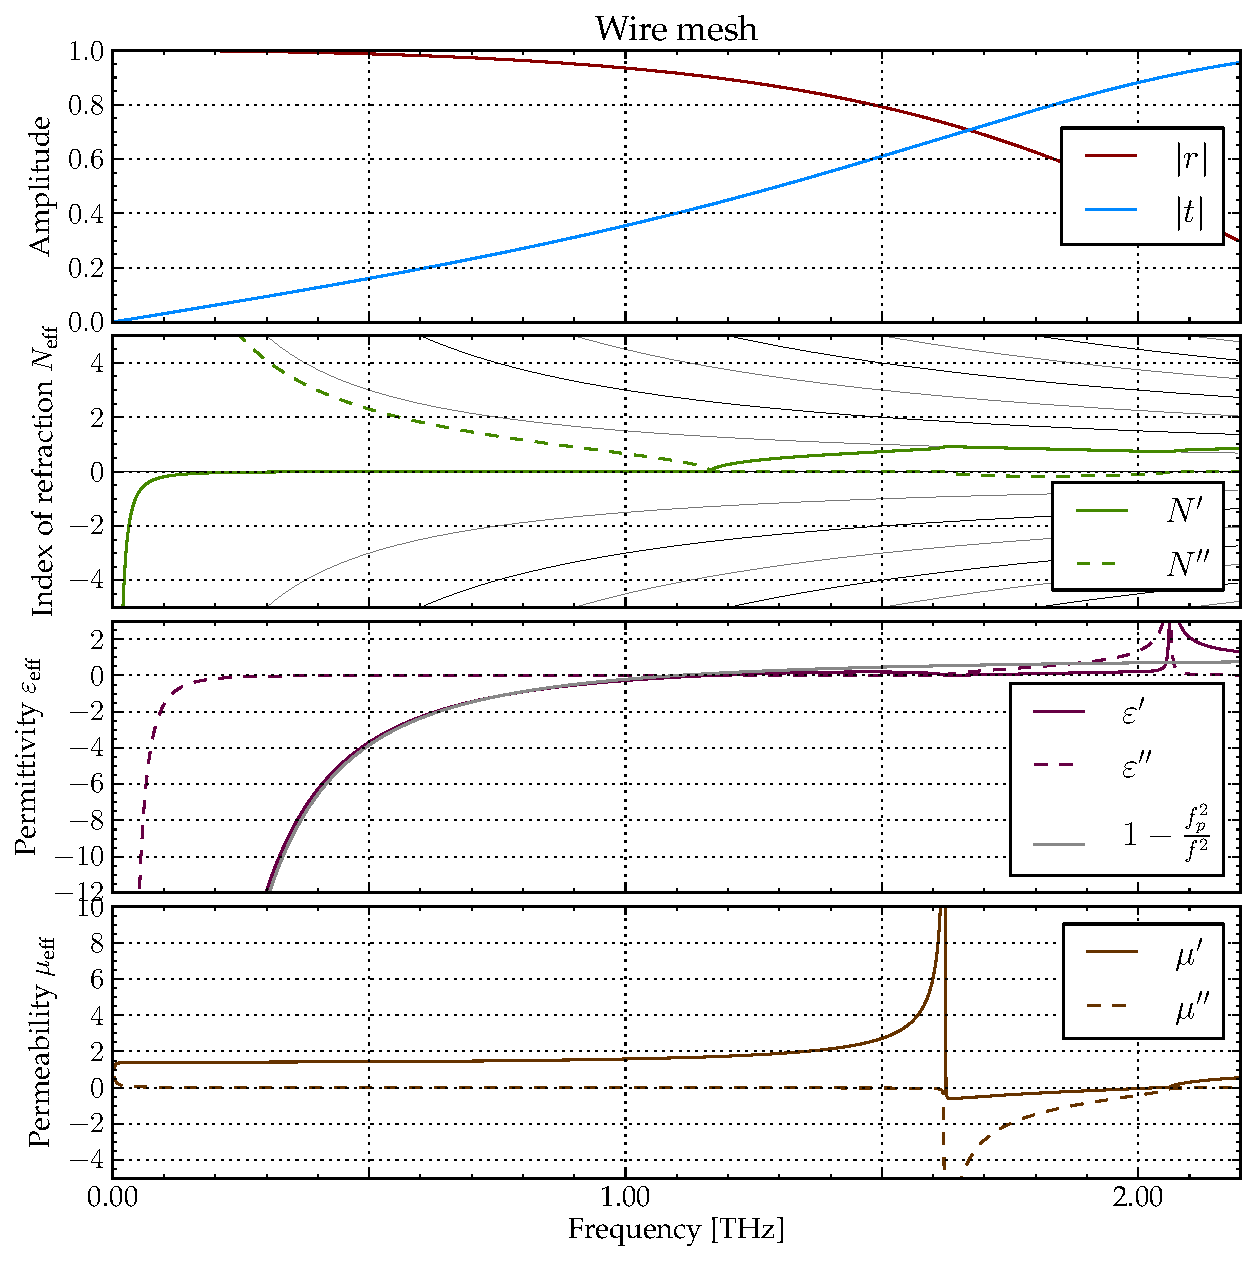
\includegraphics[width=10cm]{img/EWire_r03_FDTDwide.pdf} \end{figure} \clearpage

\add{
A dense array of thin, perfectly conductive (PEC) wires oriented along the electric field is somewhat similar to the dielectric rods of the same orientation. It might be incorrectly expected that such an array would reflect all incident radiation, i.e. it would behave just as a metallic sheet or bulk metallic block does. The simulation proves that this expectation is wrong, even when the wire density is order of magnitude higher than that would allow diffraction. The wire array allows a part of the radiation to pass through -- in other words, no wire polarizer is 100 \% perfect no matter how conductive the constituent material is.
\begin{figure}[ht]  \caption{Effective parameters of wire mesh, wires oriented both along the electric and magnetic field, with radius of $r_w = 12\;\mu$m. A realistic Drude model was used for the metal.\\ Due to high conductivity of the wires, a wrong sign of $N'$ at 0--200 GHz and of $N''$ at 1620--2080 GHz was given by computation.\\As an illustration of the plasma-like behaviour, a grey curve shows the permittivity predicted by Drude model with $f_p = 1110$ GHz.}
\label{fg_wire_fdtd} \centering 
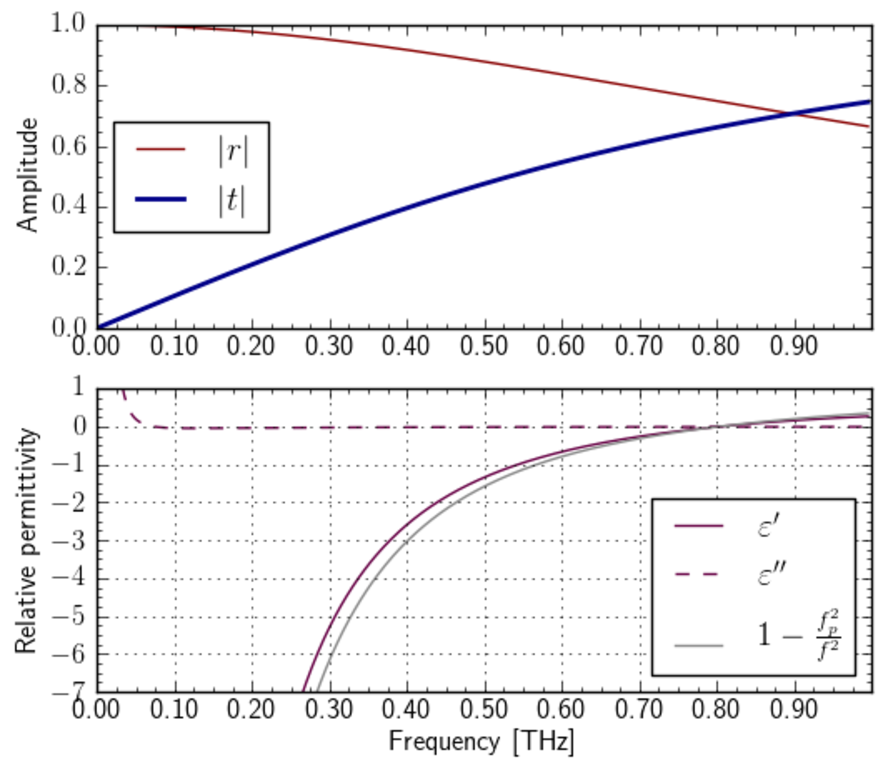
\includegraphics[width=11cm]{img/XCylWire_a100r4.pdf}
\end{figure}

Why does the transmission of a wire array differ from a metallic sheet? The key mechanism is that the current required to reflect the wave also causes the magnetic field to circulate around the wire. (This is similar to the difference between the dielectric rods $||\mathbf E$ and a homogeneous dielectric slab.) Each wire therefore behaves as a distributed inductor so it can no more entirely screen the incident electric field \cite{pendry1996extremely}. As a result, for any alternating field, always some nonzero amplitude is transmitted.

In terms of homogenized effective parameters, such a medium composed of infinite wires behaves as a "diluted metal" or plasma and its effective permittivity is finite at any nonzero frequency. The Drude model holds for low enough frequencies:
\begin{equation} \varepsilon_{\text{eff}} = 1 - \frac{f_{p}^{2}}{f^{2}} \label{eq_metaleps}\end{equation}
The permittivity is negative for frequencies below its plasma frequency $f_p$, at which $\varepsilon$ gets positive. The value of effective plasma frequency $f_p$ of the wire medium, depending on wire radius $r$ and grid spacing of $a>r$, is predicted by the analytic model\cite{maslovski2002wire} as:
\begin{equation} f_{p}^{2} = \frac{c^{2}}{2\pi \cdot a^{2} \cdot \ln\left(\frac{a^{2}}{4r \cdot (a-r)}\right)} \label{eq_fp_maslovski}\end{equation}
The more space is left around each wire and the smaller radius the wire has, the larger is its self-inductance and the lower lies the effective plasma frequency. 
Note that for a single cell, the transition from negative to positive permittivity is not accompanied by any obvious spectral feature on the reflection/transmission plot. 

We ran two series of wire array simulations (Fig. \ref{fg_omegap_a}) as a simple verification of both the FDTD algorithm and the mentioned analytic model. In the first series we kept the wire radius constant $r = 16\,\upmu$m  and changed the wire spacing $a$ (red points). For comparison, we plot in Fig. \ref{fg_omegap_a} the plasma frequency predicted by the Maslovski's analytic model\cite{maslovski2002wire} from Eq. (\ref{eq_fp_maslovski}) and by the older Pendry's model \cite{pendry1996extremely} (full and dotted lines, respectively). To test the possible error introduced by the FDTD algorithm, we ran the simulation with different resolution - results with fine $1$ $\upmu$m grid are denoted by full circles, results with coarse $4$ $\upmu$m grid with empty squares. Finally we also repeated this plot for thinner wire with $r = 8$ $\upmu$m.
\begin{figure}[ht] \caption{Comparison of numerical results and analytic model for plasma frequency $f_p$ of a wire medium. \textbf{a)} $f_p$ as a function of wire spacing, \textbf{b)} $f_p$ as a function of wire radius. } \label{fg_omegap_a} \centering 
\textbf{a)}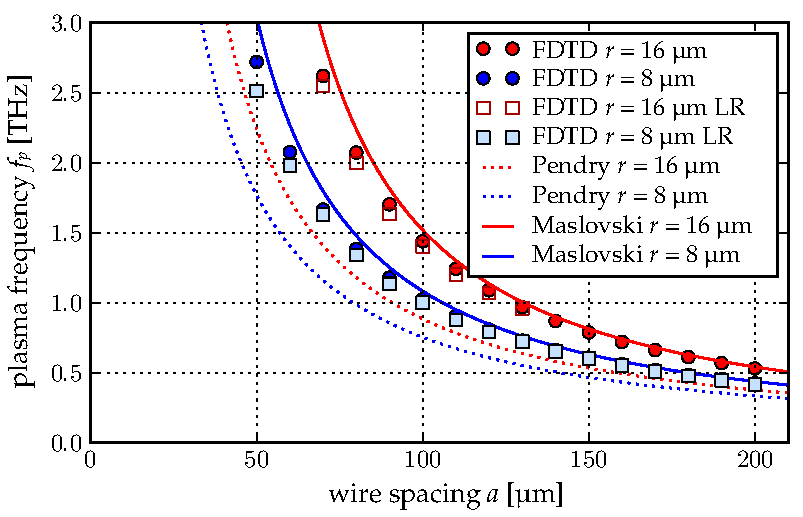
\includegraphics[width=8cm]{img/EWire_plasmaF_spacingscan.pdf}
\textbf{b)}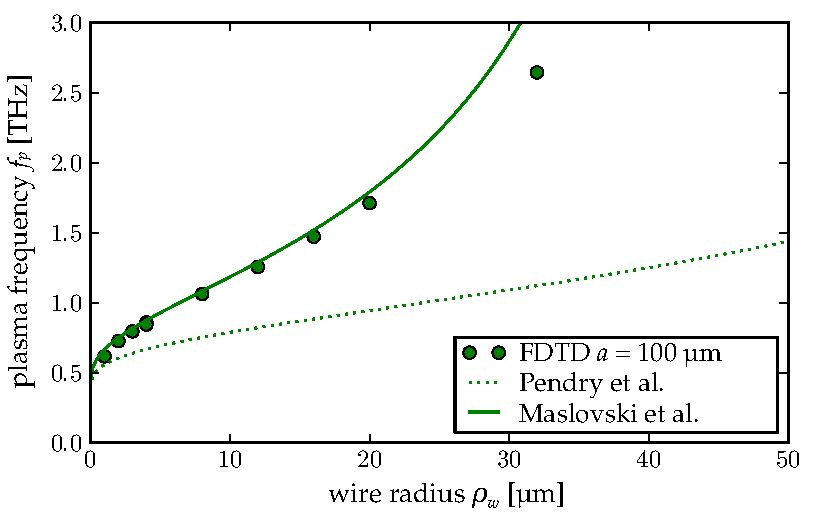
\includegraphics[width=8cm]{img/EWire_plasmaF_radiusscan.pdf}
\end{figure}

In the second series of simulations, we kept the spacing $a = 100\,\upmu$m and changed the wire radius $r$. The analytic model\cite{maslovski2002wire} and FDTD simulation give similar results (up to 5 \%) even for wire radii approaching roughly $a/4$. For thicker wires, the analytic model predicts higher plasma frequency than FDTD.  To conclude, the results of the model presented by Maslovski match the FDTD simulation with good accuracy for thin wires (where $r \lesssim a/5$). One possible application of the wire medium is in the construction of negative refractive index metamaterials, where a small negative real value of permittivity is desired.
}
%}}}

\section{Metallic strips} % references to -> % note about plasmonic particles
\section{Metallic strip pair} % references to ->
\section{Split-ring resonator} % references to ->
\section{Dielectric sphere} % references to ->
%{{{
\begin{figure} \caption{img/Sphere\_eps100\_R25\_FDTD.pdf}  \centering 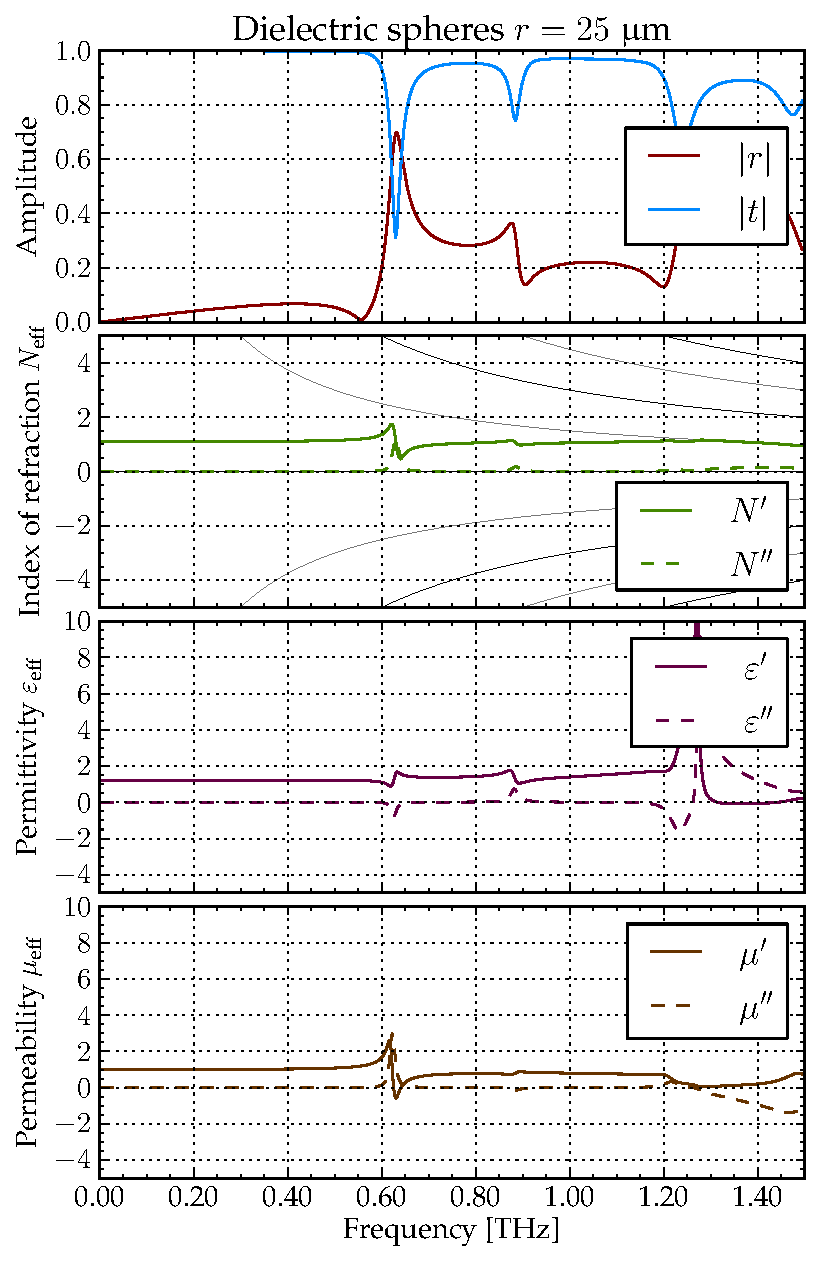
\includegraphics[width=10cm]{img/Sphere_eps100_R25_FDTD.pdf} \end{figure} \clearpage
\begin{figure} \caption{img/sphere\_Mie\_mode\_electric.pdf}  \centering 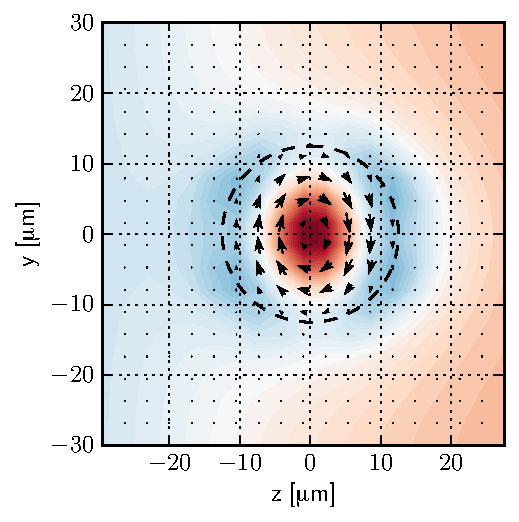
\includegraphics[width=10cm]{img/sphere_Mie_mode_electric.pdf} \end{figure} \clearpage
\begin{figure} \caption{img/sphere\_Mie\_mode\_magnetic.pdf}  \centering 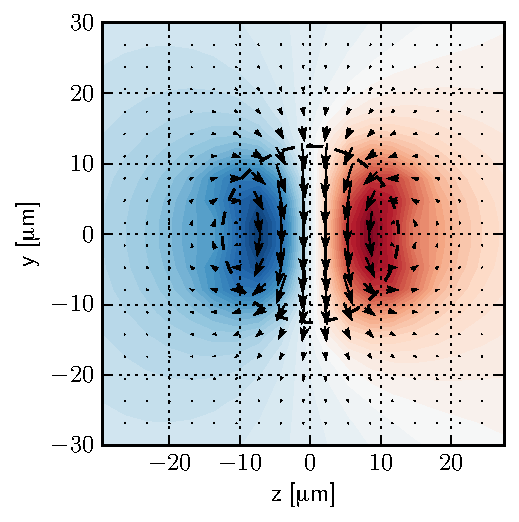
\includegraphics[width=10cm]{img/sphere_Mie_mode_magnetic.pdf} \end{figure} \clearpage
\begin{figure} \caption{img/Spheres\_FDTD\_experimentalConv.pdf}  \centering 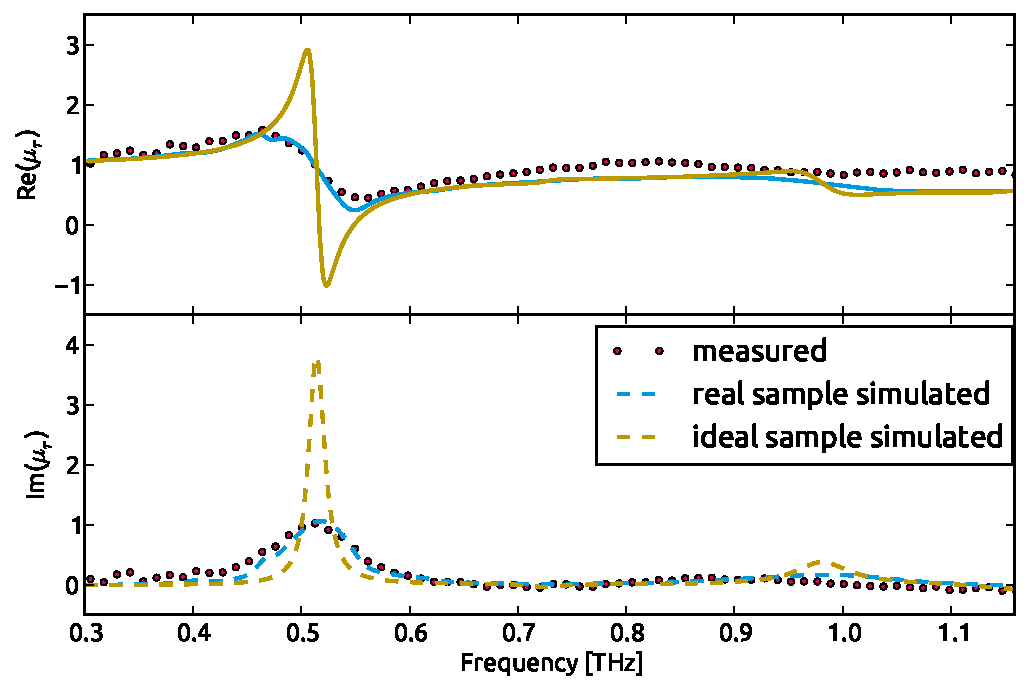
\includegraphics[width=10cm]{img/Spheres_FDTD_experimentalConv.pdf} \end{figure} \clearpage

\add{
Dielectric spheres are delimited in all three dimensions, but they have much in common with the dielectric rods. Their behaviour is closer to that of the rods with orientation parallel to the \textit{magnetic field}. The reason is that the lowest-frequency resonance of both structures is generally the magnetic one, whose circulating electric field is localised in the high-permittivity volume of the particle. Higher resonances require a significant part of the electric field to pass through surrounding air.

\begin{figure}[ht]  \caption{Effective parameters of an array of dielectric spheres \textbf{a)} Ti$\,$O$_{2}$ spheres of diameter $r=25\;\upmu$m, \textbf{b)} The same Ti$\,$O$_{2}$ spheres interlaced with thin wire mesh }
\label{fg_spheres_fdtd} \centering 
\textbf{a)}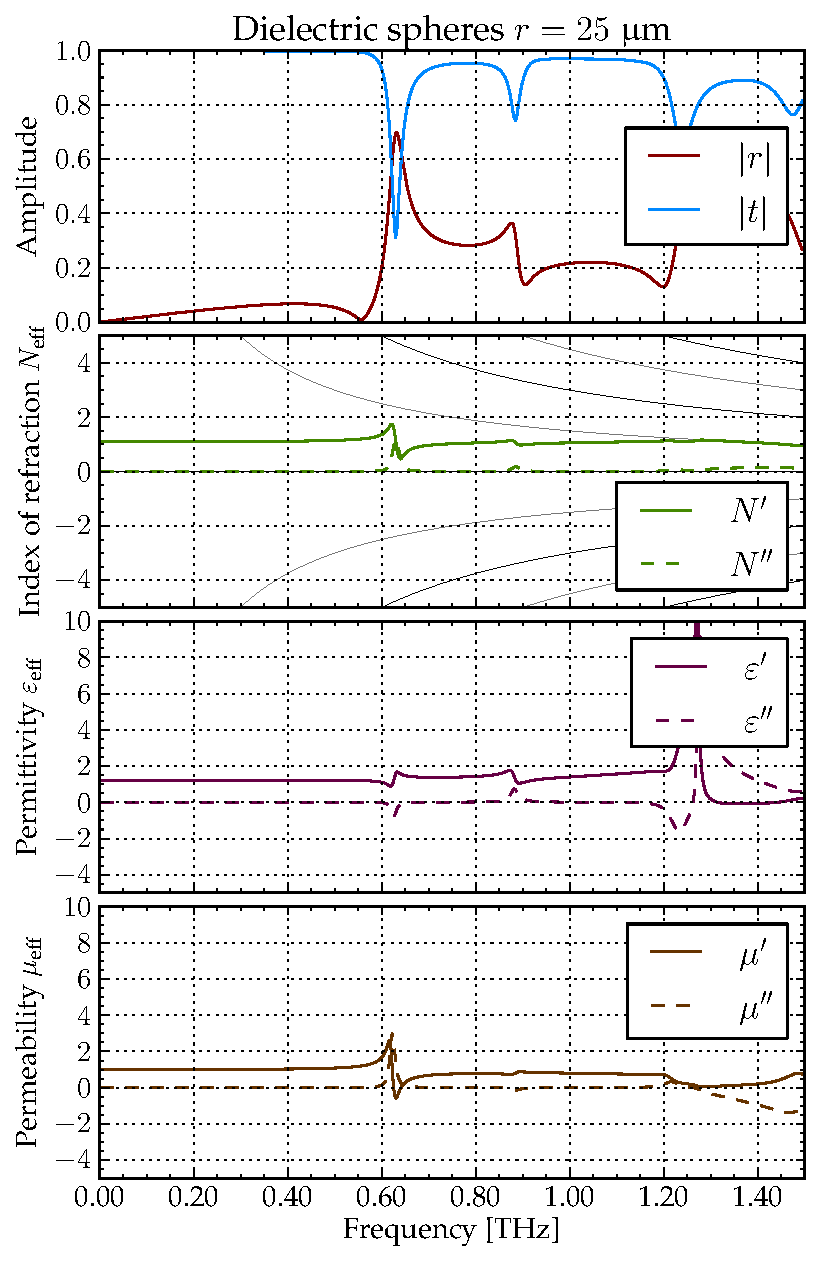
\includegraphics[width=8cm]{img/Sphere_eps100_R25_FDTD.pdf}
\textbf{b)}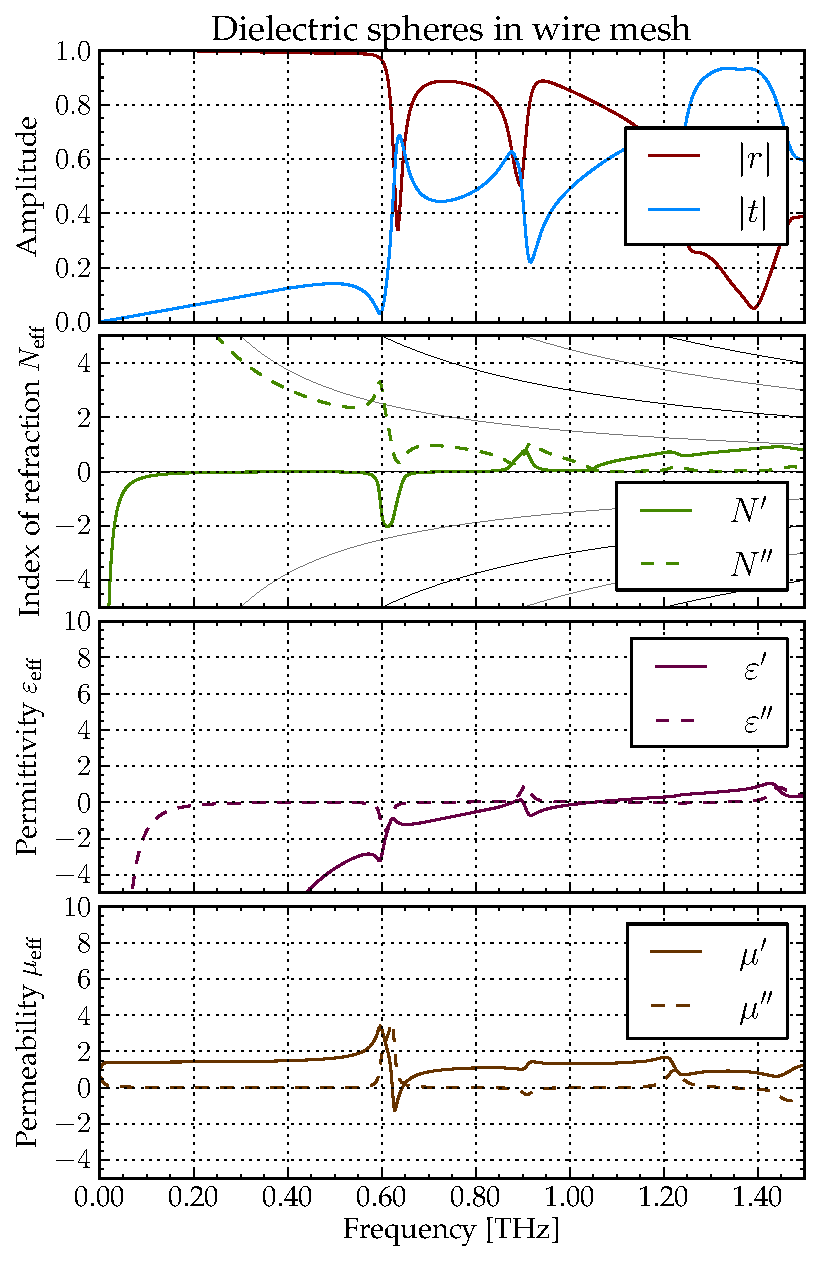
\includegraphics[width=8cm]{img/SphereWire_eps100_R25_FDTD.pdf}
\end{figure}
In contrast with previous treatment, we used a realistic model \cite{baumard1977_epsilon_TiO2} of rutile (TiO$_{2}$) for the FDTD simulations presented here to illustrate the effect of losses. The permittivity of the spheres was $\varepsilon^{\text{(1 THz)}} = 94.2+2.43\text{i}$, their diameter was set to $r=25\;\upmu$m  and their spacing along each axis was $a =100$ $\upmu$m. The resulting spectra of reflection, transmission and effective parameters are in Fig. \ref{fg_spheres_fdtd}a. A strong magnetic resonance is apparent at 330 GHz, followed by a weaker electric one at 480 GHz and another magnetic one at 670 GHz. Further resonances are gradually less visible due to lower dipole moment and also due to dielectric losses that increase with frequency. 
For completeness, we extend the frequency axis near $a/(2c) \approx 1.5$ THz, where the first Brillouin zone is reached and a classical Bragg band gap is formed.
The main difference compared to the lossless resonances discussed above (cf. Fig.~\ref{fg_rodh_fdtd}) is the continuous index of refraction, that prevents the index of refraction $N'$ near individual resonances to reach the Brillouin zone boundaries and to form clear edges of the bands. As a result, all effective parameters are continuous even near resonances and do not form separate branches.

An important property of the periodic sphere array is its \textit{isotropic} electromagnetic behaviour. It trivially follows from symmetry under any orthogonal rotation, and it also holds almost exactly under any other orientation (unless the spheres are not touching or too high frequencies are studied).

The right plot in Fig. \ref{fg_spheres_fdtd}b shows simulation results for the sphere array interlaced with a wire mesh. The wires are directed along the $x$-axis and $y$-axis, the latter orientation being included only to maintain isotropy of the structure. The wires along the $x$-axis, i.e. parallel to the electric field, have a great impact on the spectra. Most importantly, the structure is now highly reflective at low frequencies, and the resonances introduce transmission windows. (Note the previously discussed sphere array acted in opposite way!) The explanation is contained in the effective permittivity plot, where the wires introduce a region of $\varepsilon_{\text{eff}} < 0$  ranging from 0 to ca 900 GHz. More detailed study of this phenomenon is in the following section.

The magnetic resonance introduces narrow regions where $\mu_{\text{eff}} < 0$, thus leading to $N'_{\text{eff}} < 0$ and a propagation mode would occur \cite{dominec2013resonant}. The electric resonance can, on the other hand, overpower the effect of wires so that $\varepsilon_{\text{eff}} > 0$, forming a narrow band with $N'_{\text{eff}} > 0$.
%In practice the resonances are highly lossy, so only the first magnetic resonance introduces a band where the wave can propagate through several cells without being too damped. 

We performed series of experiments to measure the effective permeability  $\mu_{\text{eff}}$ spectrum in a real sample with mean sphere radius of ca. $42\;\upmu$m. The statistical deviation of the resonators size $\sigma \approx 5\;\upmu$m in the sample was unfortunately relatively broad, as was determined by means of microscopy and digital image processing. In contrast to simulations, we were able to constraint the spheres' positions to a plane only, while arranging them in a square array appeared unrealistic. We could anyway compute the single-cell permeability spectra (i. e. the yellow curve in Fig. \ref{fg_experimentalConv}) for many different resonator sizes and add them up. The resulting weighted average (blue curve) then matches the experimental data (red dots) nearly exactly. It shall be however noted that the averaged real part of $\mu_{\text{eff}}$ remained positive even with the best sieving results obtained so far.
\begin{figure}[ht]  \caption{Comparison of the effective permeability of ideal monodisperse sphere array (yellow), weighted average according to the size distribution (blue) and experimental data (red dots).}
\label{fg_experimentalConv} \centering 
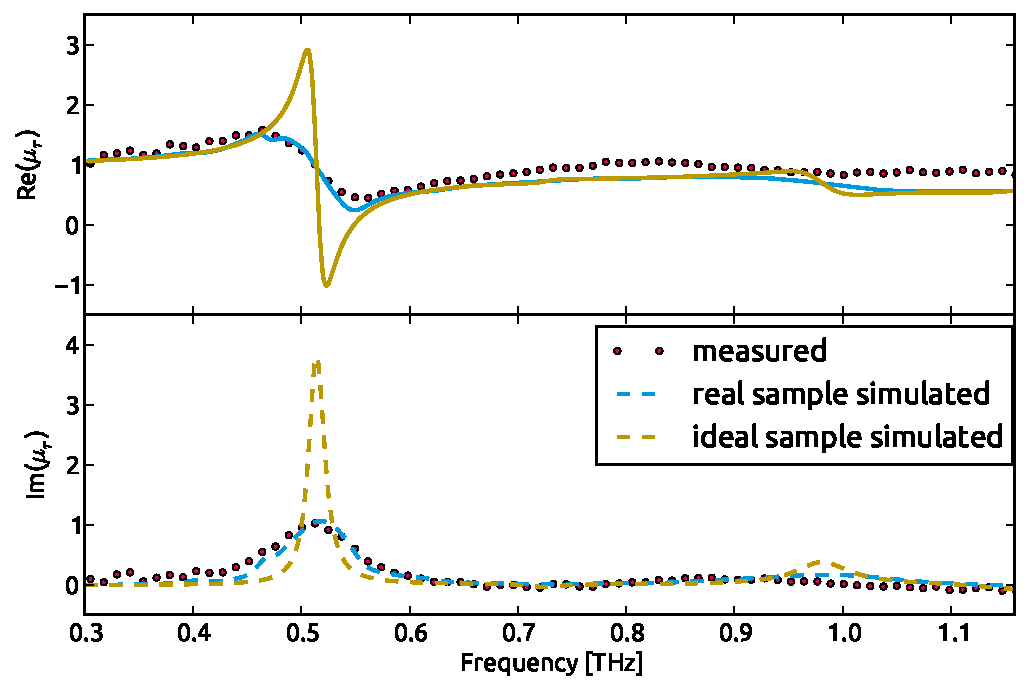
\includegraphics[width=12cm]{img/Spheres_FDTD_experimentalConv.pdf}
\end{figure}
}
%}}}
%% TODO? E-mail: Add the x, y, z, size scans of the ellipsoids%{{{
%> On 19 Mar 2014, at 15:57, <dominecf@fzu.cz>
%> wrote:
%>
%>> Dear Oleg and all,
%>> the frequency dependence of the Mie modes in an ellipsoid is
%>> nontrivial.
%>> Maybe some skilled mathematician could find the analytic expression,
%>> but I
%>> guess its evaluation would require a computer anyway. As an interesting
%>> numerical experiment with FDTD, I ran three scans over the X-, Y- and
%>> Z-
%>> semiaxes of a TiO2 ellipsoid, fixing the remaining semiaxes to 15 um.
%>> The
%>> ellipsoid's X-axis was oriented parallel to the electric field, the
%>> Z-axis
%>> pointed in the wave propagation direction.
%>>
%>> The results attached, best expressed by the dielectric loss spectra in
%>> bilogarithmic plot, show that the first (magnetic) mode is roughly
%>> proportional to X**(-0.4) and Z**(-0.4), while the dependence on the
%>> Y-size is even slower, similar to Y**(-0.2).
%>>
%>> The second Mie mode is more sensitive to the Z-size as Z**(-0.7), while
%>> the other sizes scale very slowly, X**(-0.15), Y**(-0.15).
%>>
%>> In all cases, the exponents of X, Y and Z~dependencies should sum up to
%>> -1, which is the obvious rule for the frequency dependence when all
%>> axes
%>> are scaled simultaneously!
%>>
%>> Note that these estimated exponents are roughly valid only near the
%>> spherical shape, ie. when X~Y~Z. As a matter of fact, the tuning curves
%>> are not straight in the log-log plots. Naturally when one ellipsoid
%>> dimension is much lower than the other two, its role becomes more
%>> pronounced.
%>>
%>> Now we are coming to the big conclusion: Near the spherical shape, the
%>> difference of exponential slope between X- and Y- elongation is
%>> (0.4-0.2)=0.2. Therefore, (15./12.)**(0.4-0.2) gives a reasonable
%>> factor
%>> of 1.0456 difference for the resonant frequencies of the magnetic mode.%}}}

\section{SRRs and spheres in wire grid} % references to ->
%{{{
\begin{figure} \caption{img/SphereWire\_eps100\_R25\_FDTD.pdf}  \centering  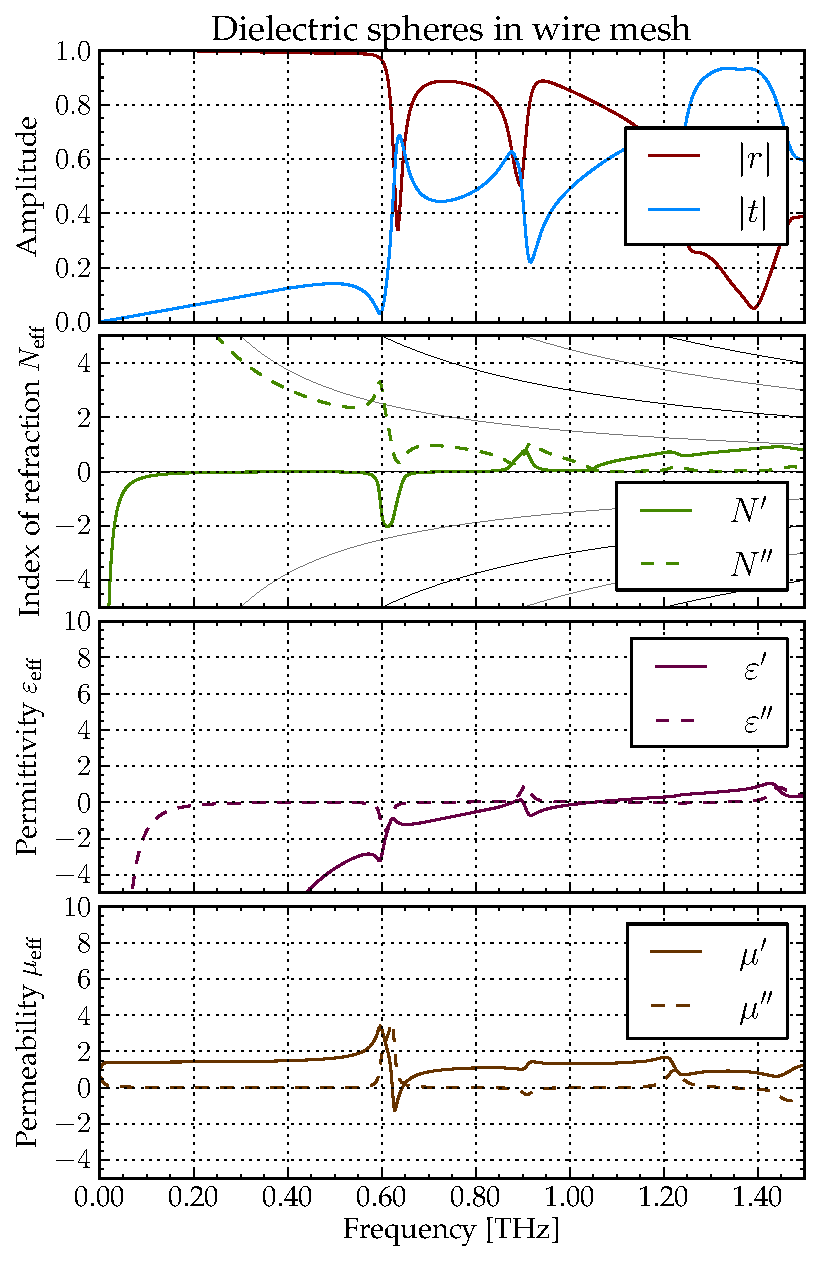
\includegraphics[width=10cm]{img/SphereWire_eps100_R25_FDTD.pdf} \end{figure} \clearpage
\begin{figure} \caption{SphereWire sketch}  \centering  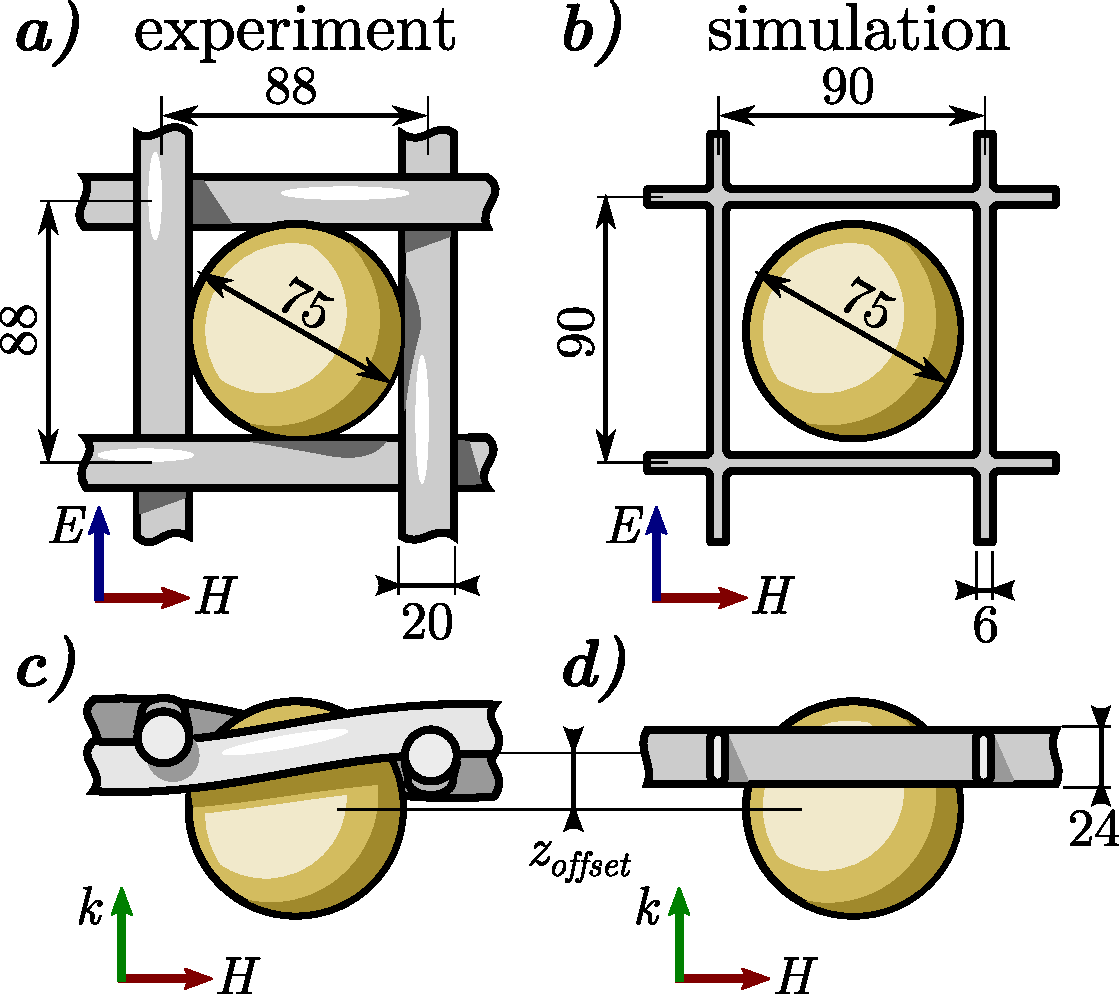
\includegraphics[width=10cm]{img/SphereWire_sketch.pdf} \end{figure} \clearpage
%}}}
\section{Dielectric rods parallel to magnetic field} % references to ->
%{{{
\begin{figure} \caption{img/HRods\_eps012\_R12\_PWEM.pdf}  \centering 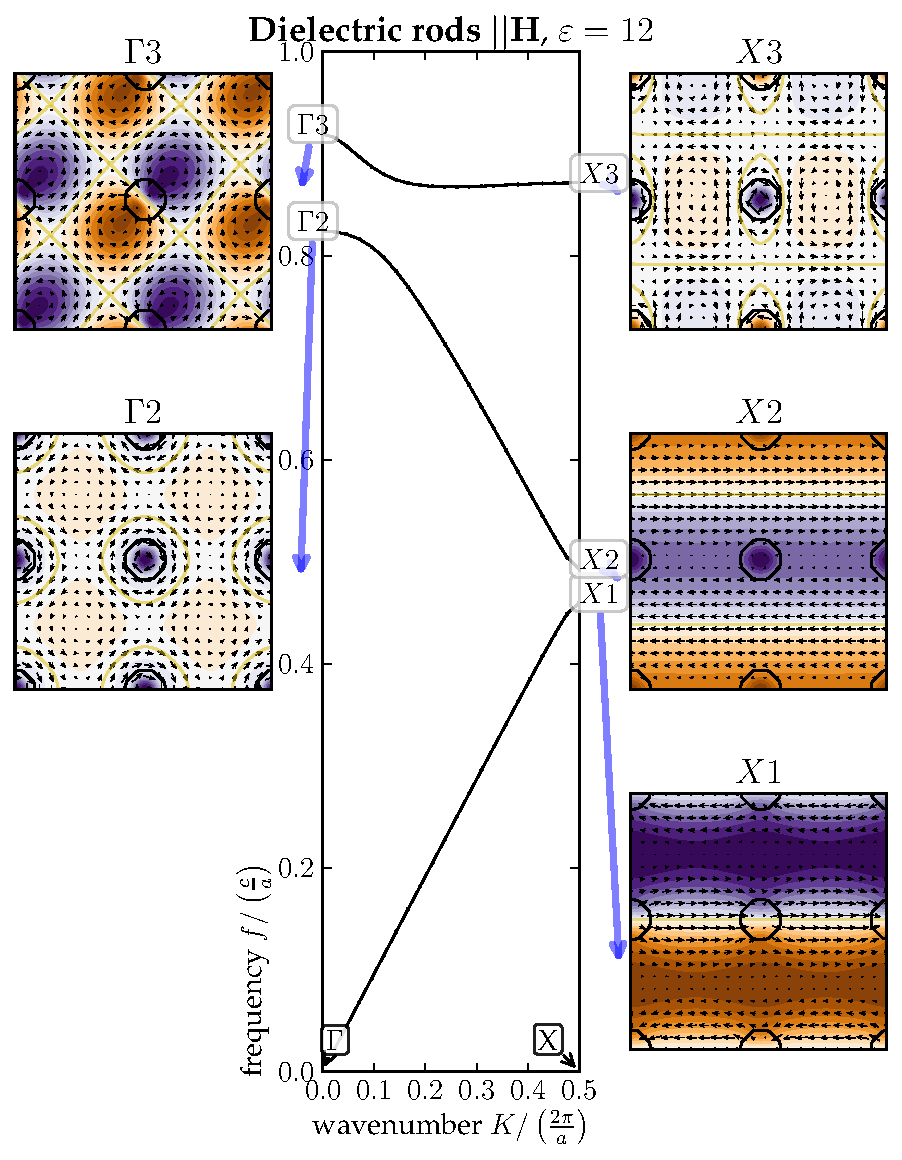
\includegraphics[width=10cm]{img/HRods_eps012_R12_PWEM.pdf} \end{figure} \clearpage
\begin{figure} \caption{img/HRods\_eps100\_R12\_FDTD.pdf}  \centering 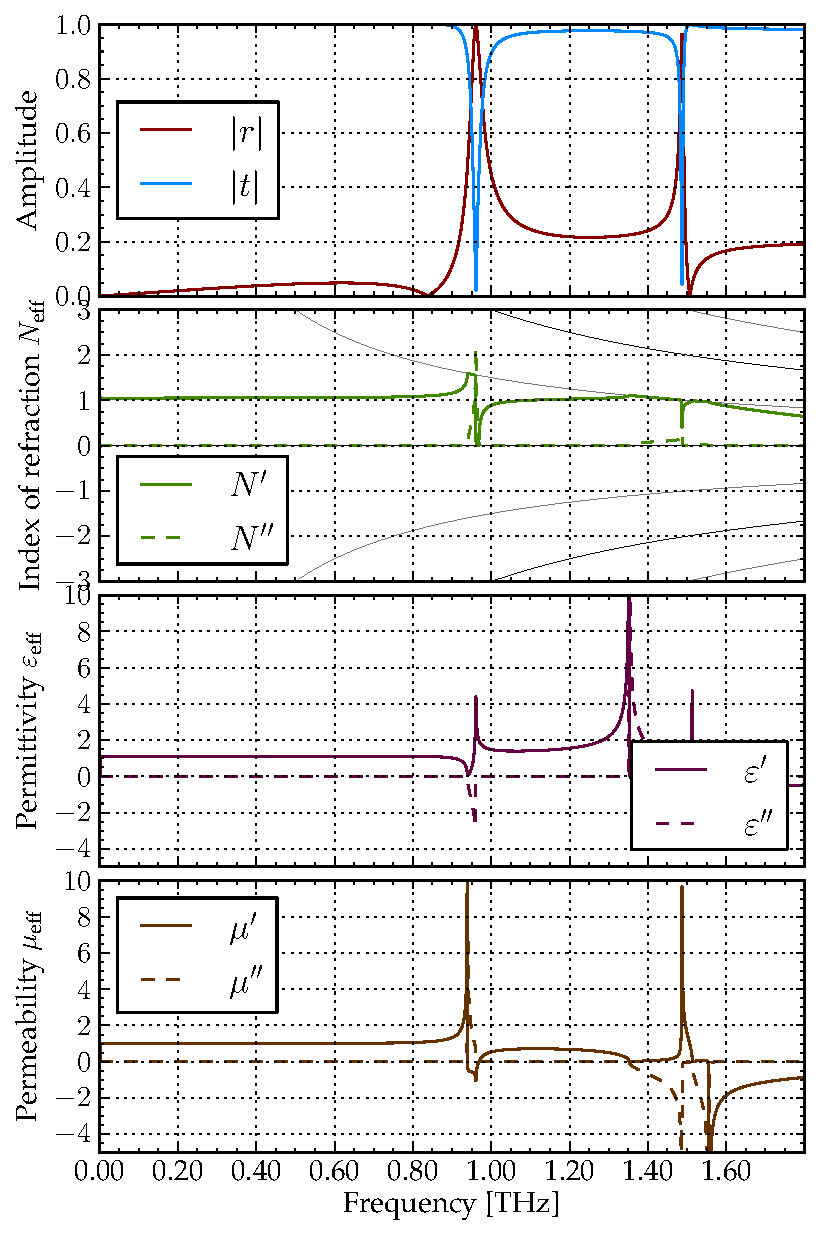
\includegraphics[width=10cm]{img/HRods_eps100_R12_FDTD.pdf} \end{figure} \clearpage
\begin{figure} \caption{img/HRods\_eps100\_R12\_PWEM.pdf}  \centering 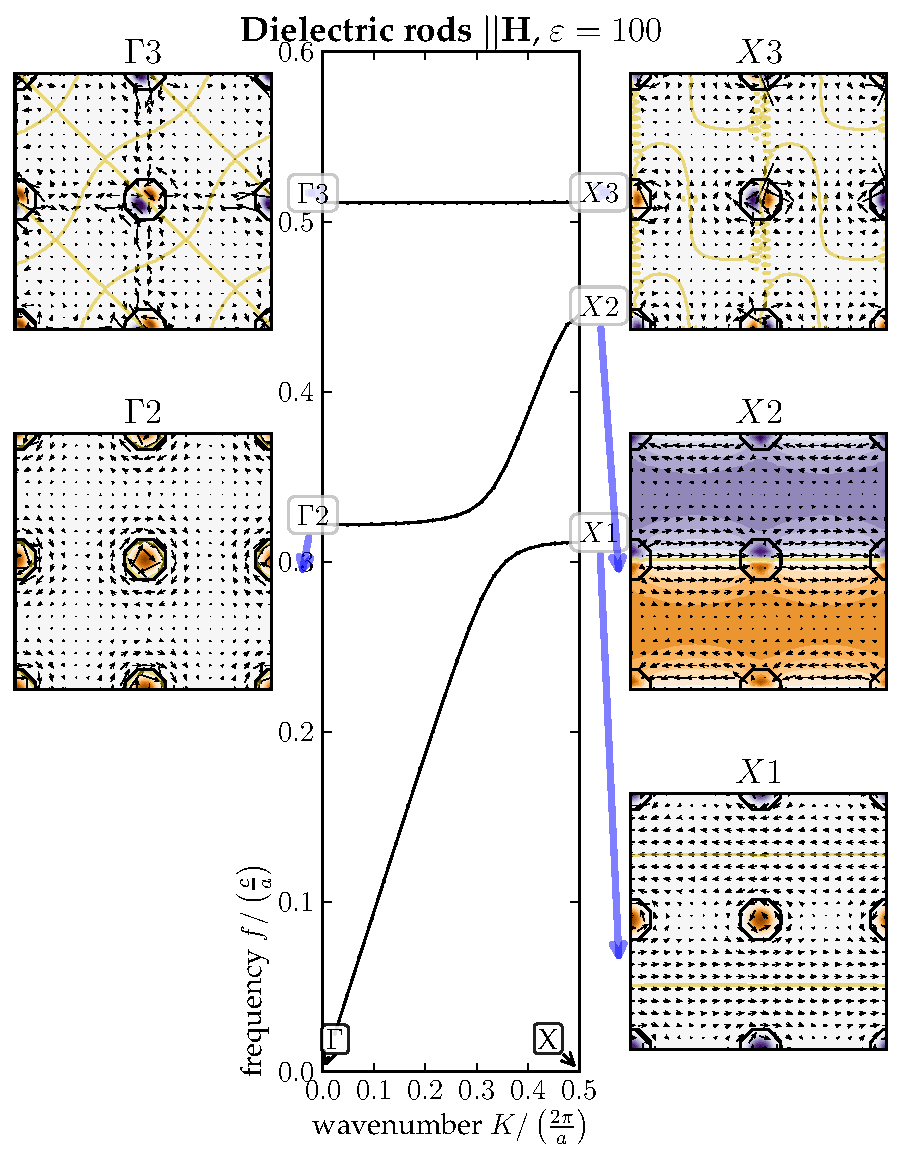
\includegraphics[width=10cm]{img/HRods_eps100_R12_PWEM.pdf} \end{figure} \clearpage
%\begin{figure} \caption{img/HRods\_sketch.pdf}  \centering 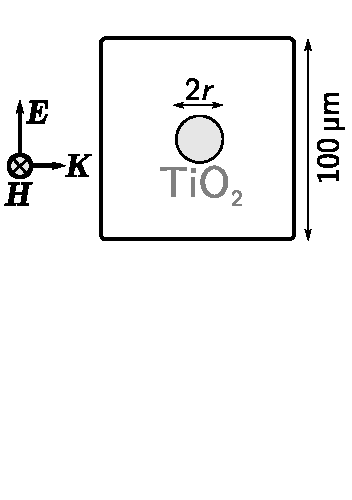
\includegraphics[width=10cm]{img/HRods_sketch.pdf} \end{figure} \clearpage ## nonexistent
% todo? analytic Mie resonance frequency? -> OBrien&Pendry2002, szabos etc
\add{
Are there also different, non-Bragg, mechanisms that can create band gaps?


We would not indeed pose this question if its answer were negative. It is closely related to the \textit{internal resonances} based on non-propagating evanescent fields in the structure. The operation of all sorts of left-handed metamaterials  relies on these resonances. We conjecture such resonances may never occur in 1-D dielectric structures, so their study requires a simulation of a 2-D or 3-D structure.
% Todo elaborate the idea of nonBragg gap <-> nonradiative fields in structure <-> permittivity/permeability resonance
% Note that in 1-D dielectric PhC, all fields are propagating, none evanesecnt
% Big question: Can one approximate a metamaterial by ENG/DNG/MNG/DPS 1-D PhC??
\begin{figure}[ht] \caption{Dispersion curves for dielectric rods aligned parallel to magnetic field. The side plots show the shape of the fields in the $(x,z)$ plane, at the frequencies of the band edges. The magnetic field is plot as color map and the electric field is represented by vectors. The rod radius was chosen to 12 \% of the period. \textbf{a)} On the left, a relatively low permittivity $\varepsilon = 12$ places the magnetic resonance above the first Bragg band gap. \textbf{b)} For high permittivity dielectric $\varepsilon = 100$, the magnetic resonance forms the first band gap. } \label{fg_rodh} \centering 
\textbf{(a)}	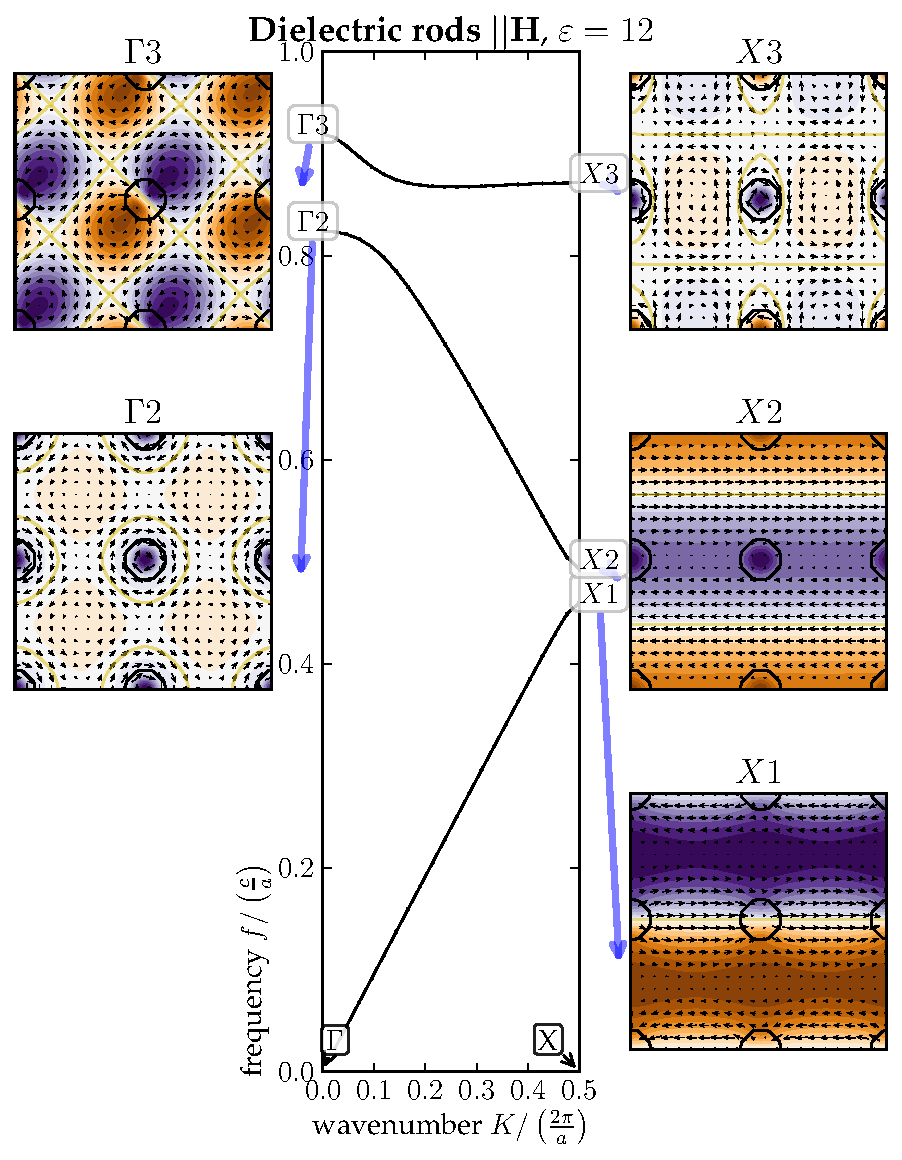
\includegraphics[width=8cm]{img/HRods_eps012_R12_PWEM.pdf}
\textbf{(b)}	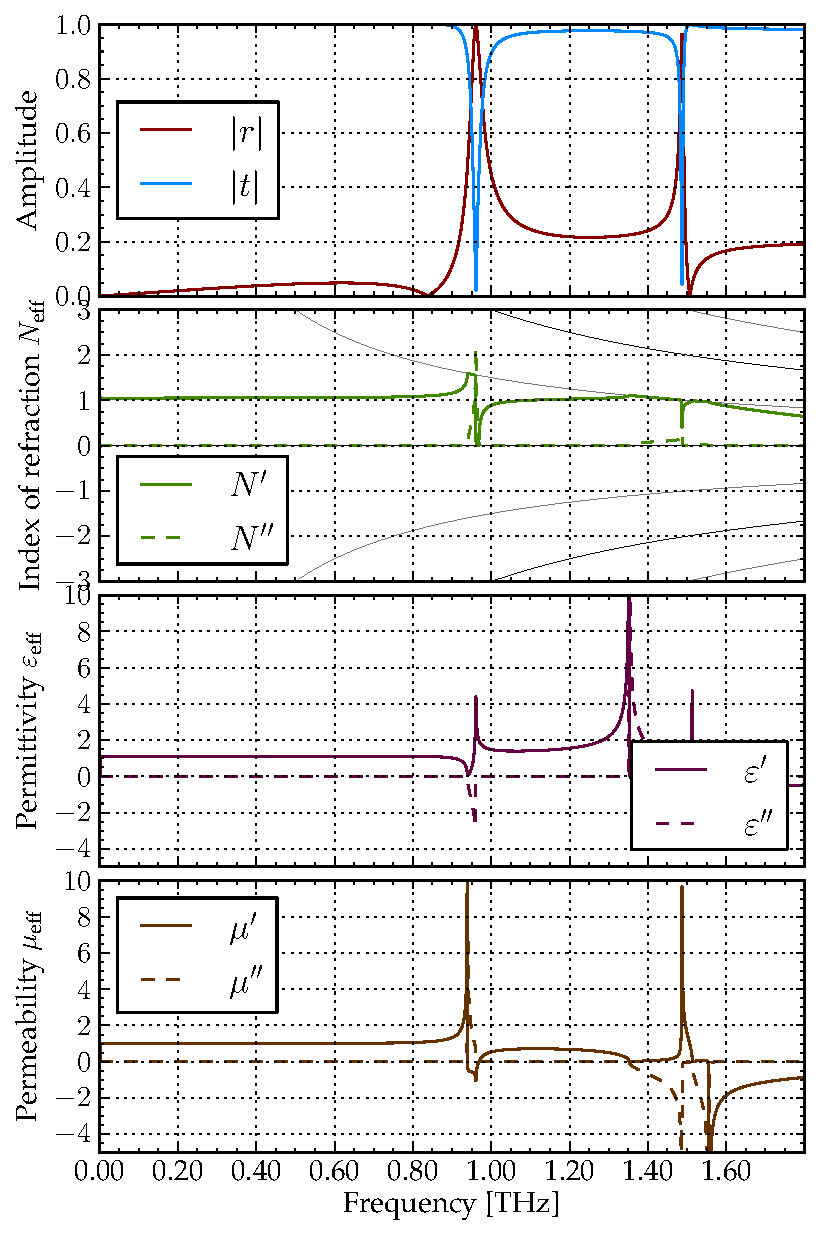
\includegraphics[width=8cm]{img/HRods_eps100_R12_FDTD.pdf}
\end{figure}

Probably the simplest example of such structures is a periodic array of high-permittivity dielectric rods, aligned parallel to the $y$-axis. (We use the convention that the structure is excited by a plane wave source with $\mathbf E || \mathbf x$, $\mathbf H || \mathbf y$ and the wave propagates along the $z$-axis). % dubious - the E, H have many directions in the unit cell; better  to write "TM"/"TE"? But this would confuse with nonperp incidence!
The inhomogeneity of the structure along the $x$-axis allows the electric field to circulate along the rod -- or, more precisely, the $\mathbf E$ field can now be decomposed into purely \textit{planar} part known from the previous section, and a purely \textit{circulating} part, that induces a magnetic flux near the rod axis. The circulating electric field is clearly visible on both plots in Fig. \ref{fg_rodh}, where all nonzero components of the fields ($H_y$, $E_x$ and $E_z$) are depicted. 

% discuss why this is not true: each lorentzian introduces delta mu -> so the low-frequency permeability of rod array should be > 1? Attracted to a magnet?
This new type of resonance is known as a \textit{magnetic Mie resonance}, \cite{obrien2002photonic, nemec2009tunable, yahiaoui2009broadband, yahiaoui2011tunable}. Unlike the Bragg gaps, it can be observed also in a single rod in free space. Being a function of the frequency of the incident wave, the magnetic dipole moment of the free-standing dielectric rod follows the characteristic Lorentzian shape of its \textit{resonance curve}. Below the resonance the magnetic dipole moment of the resonator goes to strongly positive values, while in a narrow region above the resonance it is strongly negative. How does this behaviour change if we arrange the rods in an infinite periodic array? 

\add{

The results from a PWEM computation are plot in Fig. \ref{fg_rodh}. To obtain comparable dispersion curves in Fig. \ref{fg_rodh_fdtd}, we employed the FDTD simulation and the effective parameter retrieval described above. The main differences are that in Fig. \ref{fg_rodh_fdtd} we plot the frequency $f$ on the horizontal axis and we also use the effective index of refraction $N_{\text{eff}} := K\cdot \frac{c}{2\pi\,f}$ instead of the wavenumber $K$. One advantage of this representation is that $N_{\text{eff}}$ should be compliant with the Kramers-Kronig relations. This criterion always gives \textit{only one} correct solution on how to unfold $K$ to obtain realistic $N_{\text{eff}}$. 
In the simulation, the rod spacing (or, lattice constant) $a$ was 100 $\upmu$m, so the normalised frequency unit is $c/a = 3$ THz. The frequency range from 0 to 1.8 THz was therefore chosen the same as in Fig. \ref{fg_rodh}b. 
Note the first resonance shows pronounced resonant shape in the plot of permeability, which is typical of magnetic Mie resonances. In a very narrow region 960-970 GHz, the permeability $\mu_{\text{eff}}$ is real and negative. 
Apart from $N_{\text{eff}}$, the FDTD computation gives also the effective wave impedance $Z_{\text{eff}}$, which is a complementary information we need to compute the effective permittivity $\varepsilon_{\text{eff}}$ and the effective permeability $\mu_{\text{eff}}$:

\begin{equation} \varepsilon_{\text{eff}} = N_{\text{eff}}/Z_{\text{eff}}, \quad\quad\quad\quad \mu_{\text{eff}} = N_{\text{eff}}\cdot Z_{\text{eff}}.
\label{eq_epsmu}\end{equation}

\begin{figure}[ht]  \caption{Effective parameters of an array of dielectric rods $||\mathbf H$ with same parameters as in Fig. \ref{fg_rodh}b (i.e. radius of  12 \% of the period and permittivity $\varepsilon = 100$). Complex reflection $r$ and transmission $t$ spectra allow to compute the effective index of refraction, impedance (not shown), permittivity and permeability. Thin grey lines indicate the Brillouin zone boundaries.}
\label{fg_rodh_fdtd} \centering 
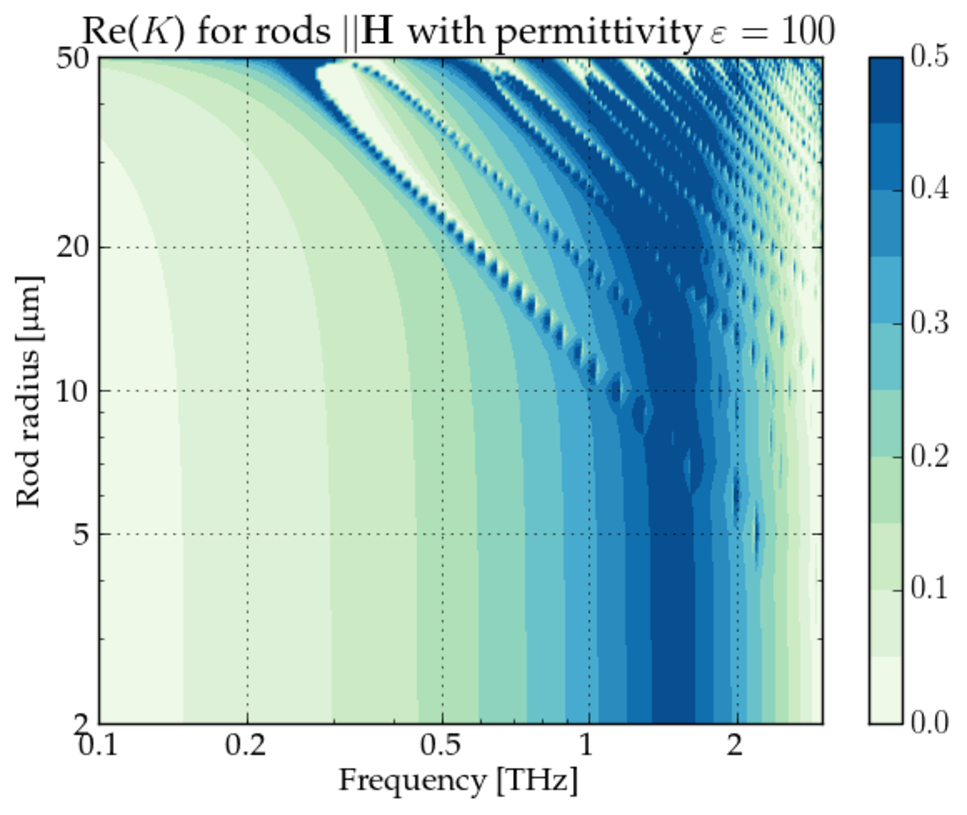
\includegraphics[width=8cm]{img/old/HRods_eps100_radiusscan.pdf}
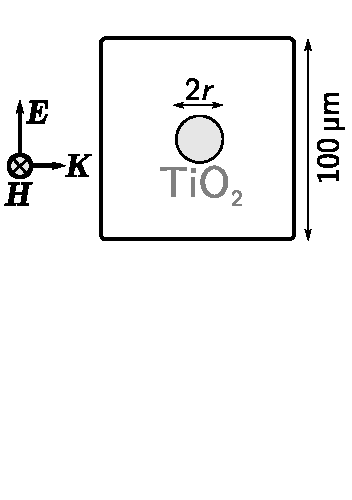
\includegraphics[width=4.5cm]{img/HRods_sketch.pdf}
\end{figure}

Other Mie resonances are located at higher frequencies. As a general rule for similar structures, the odd-numbered resonances have magnetic dipole moment (along the rod axis), whereas the even-numbered resonances have electric dipole moment (perpendicular to the rod axis). The reason is that electric dipole moments in odd resonances are suppressed due to antisymmetric shape of the mode; naturally the same holds for the magnetic moments in the even resonances.

The frequency of the Mie resonances is not significantly influenced by the photonic bands. Therefore, in order to understand the resulting band structure and its dependence on parameters, one has to disentangle which band gaps are due to Bragg reflection and which correspond to magnetic or electric Mie resonances. This is much easier knowing the spectra of $\varepsilon_{\text{eff}}$ and $\mu_{\text{eff}}$, as provided by FDTD in Fig. \ref{fg_rodh_fdtd}.
\begin{figure}[ht] \caption{The spectra of the wavenumber $K$ for different rod radii and two different rod permittivities. The wavenumber plot is folded so it ranges from 0 to 0.5, where $K\approx 0$ and $K\approx 0.5$ correspond to band gaps. \textbf{a)} Medium-permittivity rods with $\varepsilon = 12$, \textbf{b)} high-permittivity rods with $\varepsilon = 100$.  } \label{fg_hbar_radiusscan} \centering 
\textbf{a)}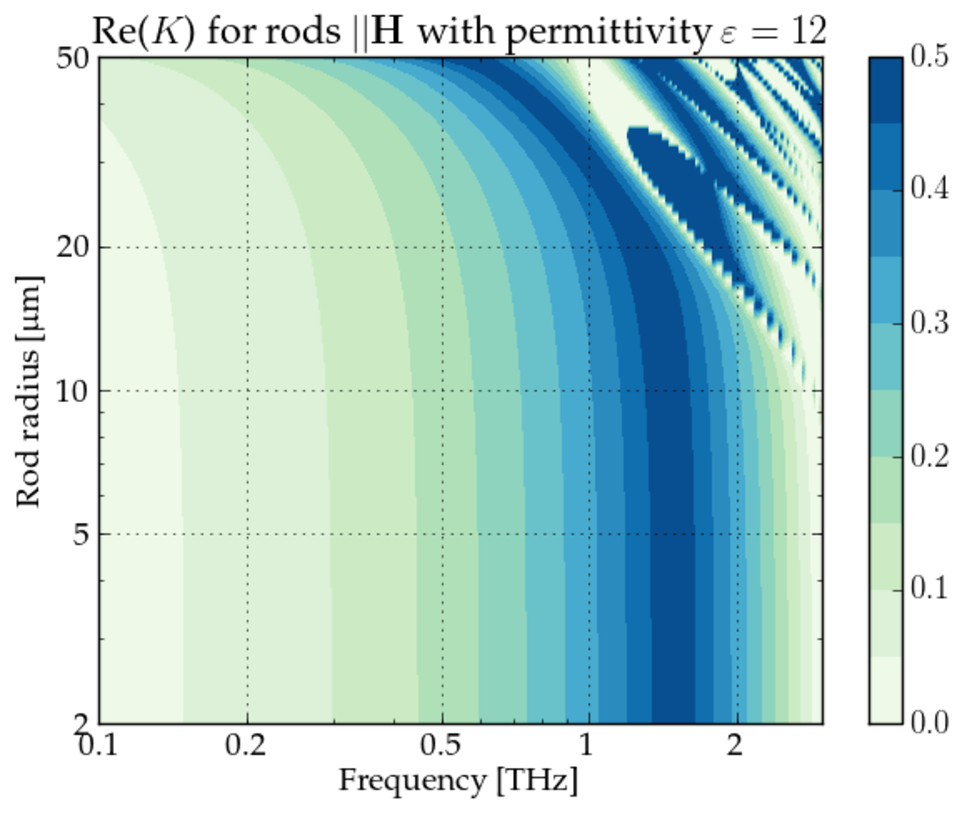
\includegraphics[width=8cm]{img/old/HRods_eps012_radiusscan.pdf}
\textbf{b)}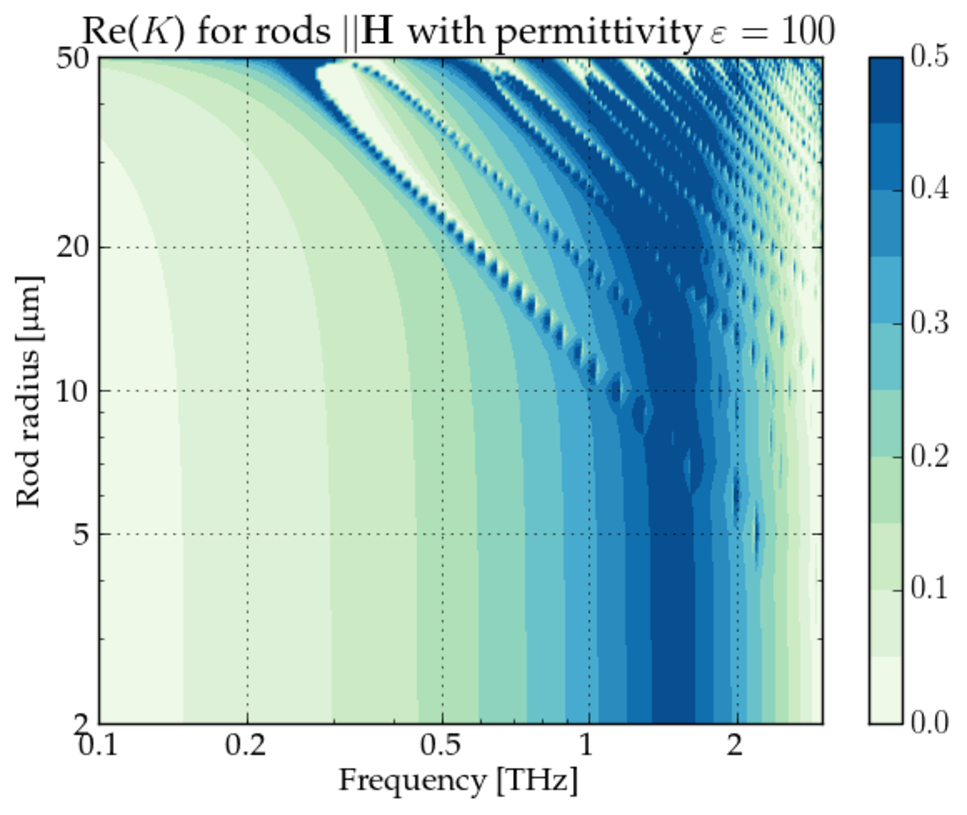
\includegraphics[width=8cm]{img/old/HRods_eps100_radiusscan.pdf}
\end{figure}

The photonic crystals composed of square lattice of dielectric rods have been examinated thoroughly since early 90s \cite{plihal1991two, pendry1992_transfer_matrix}. The permittivity of the constituent materials was rather low, corresponding to the optical or near-infrared frequencies, where the suitable materials usually have permittivity $\varepsilon < 12$. By parametric scans we could prove that for rod permittivity below 60 or even 80, the individual resonance is always located at higher frequency than the Bragg gap. Little, if any, attention was therefore paid to different nature of the higher resonances and most publications focused on properties and applications of the Bragg band gap.

The situation is different in the terahertz range, as the lattice of the crystalline solids often exhibits optical phonons at frequencies between 5 and 20 THz. The permittivity of many materials turns out to be much higher for frequencies below these resonances. This enables to conceive structures composed e.g. of titanium dioxide \cite{baumard1977_epsilon_TiO2} with $\varepsilon^{\text{THz}} \approx 92$ or of ferroelectrics with $\varepsilon^{\text{THz}}$ even orders of magnitude higher \cite{skoromets2011tuning}. The price to be paid for this advantage in the THz range are the relatively high losses caused by the lattice vibrations.
}

\begin{figure}[ht] \caption{Behaviour of the rods $||\mathbf E$, with permittivity $\varepsilon = 100$ and radius $r=11\;\upmu$m.\\
\textbf{a)} Band diagram and modes from PWEM. 
\textbf{b)} The effective parameters computed using FDTD confirm the previous results.  } \label{fg_erod_radius11} \centering 
\textbf{a)}	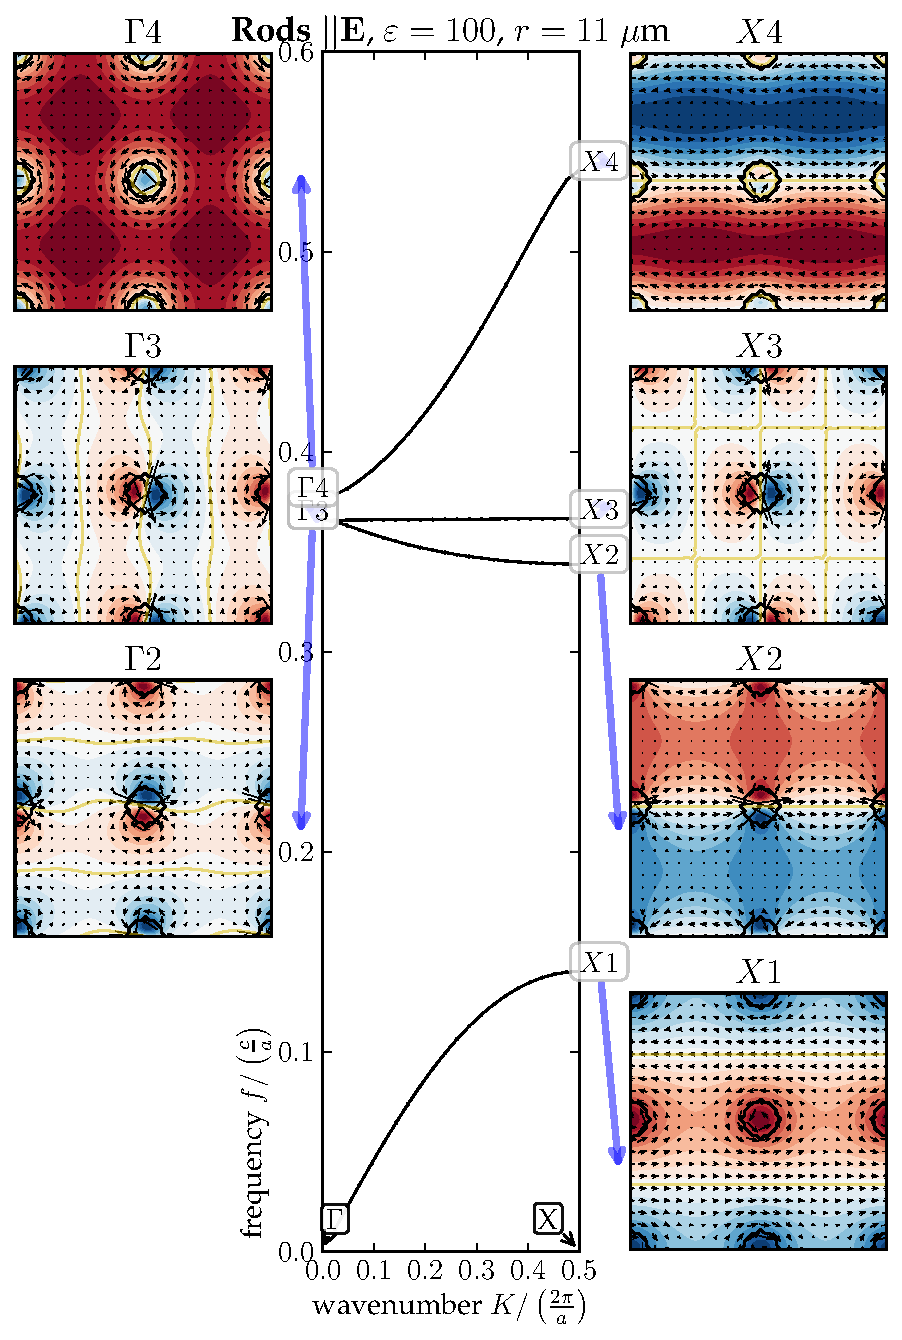
\includegraphics[width=8.5cm]{img/ERods_eps100_R11_PWEM.pdf}
\textbf{b)}	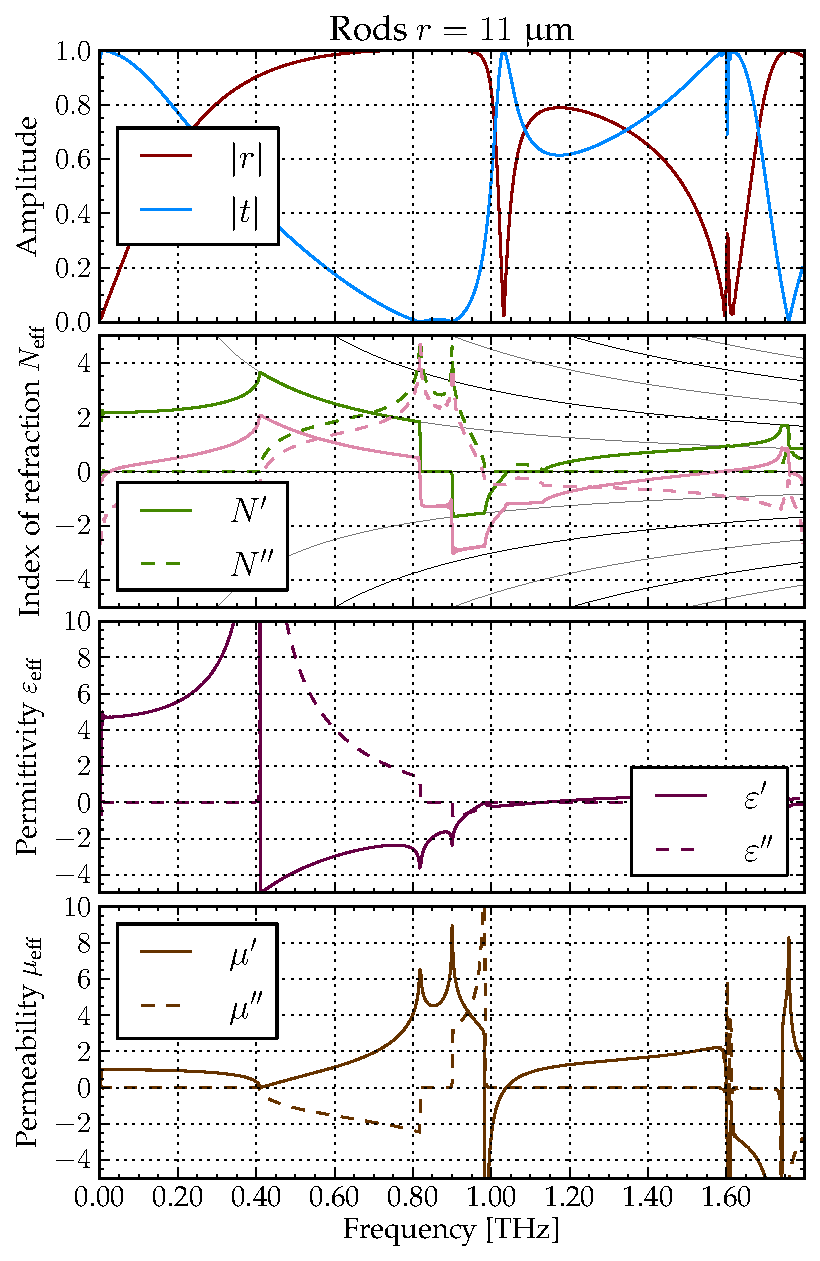
\includegraphics[width=8.0cm]{img/old/ERods_eps100_11um_FDTD.pdf}
\end{figure}

}

%}}}
\section{STO bar TODO} % references to ->
%{{{
\begin{figure} \caption{img/STOBar\_photo\_narrow.pdf}  \centering 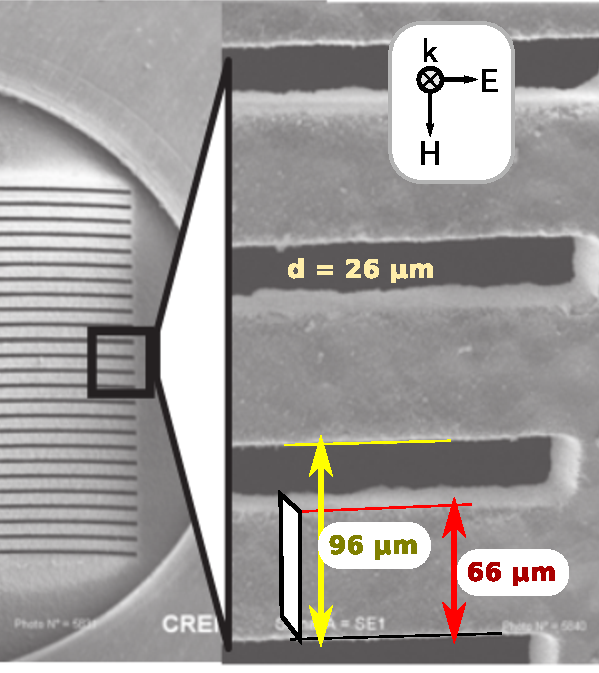
\includegraphics[width=10cm]{img/STOBar_photo_narrow.pdf} \end{figure} \clearpage
\begin{figure} \caption{img/STOBar\_photo.pdf}  \centering 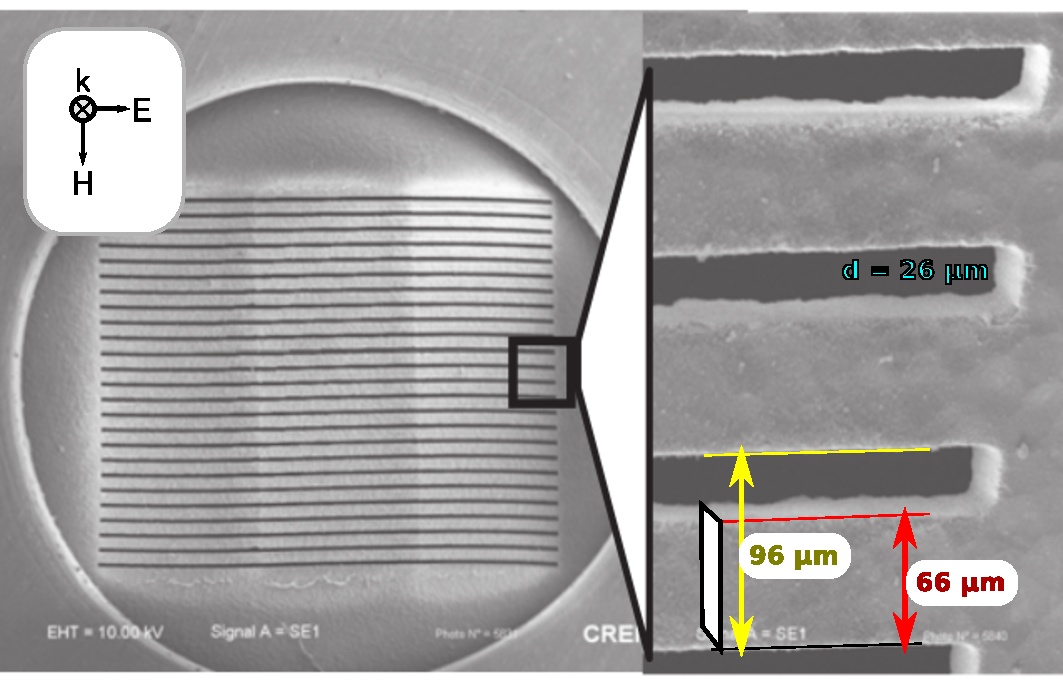
\includegraphics[width=10cm]{img/STOBar_photo.pdf} \end{figure} \clearpage
\begin{figure} \caption{img/STObar\_rt.pdf}  \centering 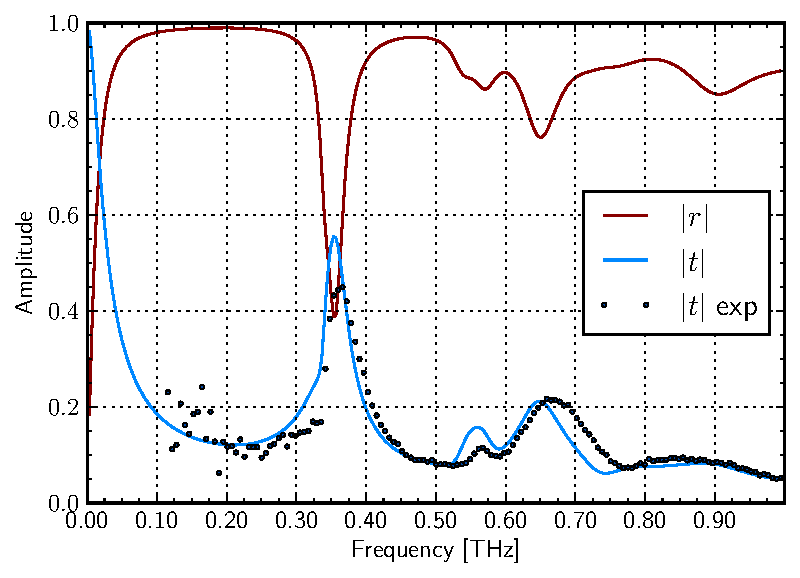
\includegraphics[width=10cm]{img/STObar_rt.pdf} \end{figure} \clearpage
\begin{figure} \caption{img/EBars\_STO\_sketch.pdf}  \centering 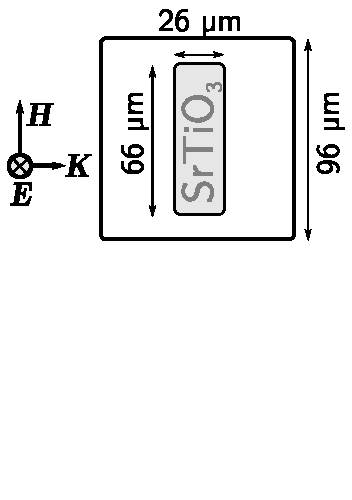
\includegraphics[width=10cm]{img/EBars_STO_sketch.pdf} \end{figure} \clearpage
%}}}
\section{Dielectric rods parallel to electric field} % references to ->
%{{{
% TODO refereence  also to \cite{valdivia2012} and \cite{shi2007}






%}}}


\mdf{%{{{ FROM SHORT.pdf
\begin{figure}[ht] \caption{The spectra of the wavenumber $K$ for different rod radii and two different rod permittivities, analogical to Fig. \ref{fg_hbar_radiusscan} except for different orientation. \textbf{a)} Medium-permittivity rods with $\varepsilon = 12$, \textbf{b)} high-permittivity rods with $\varepsilon = 100$.  } \label{fg_ebar_radiusscan} \centering 
\textbf{a)}	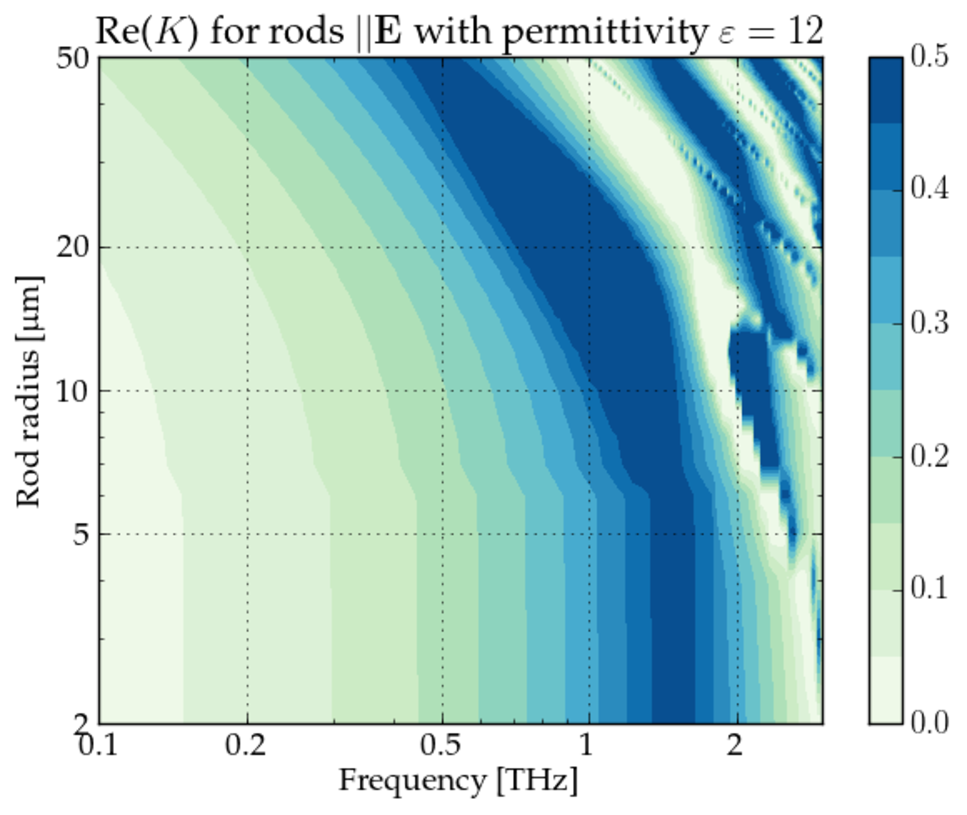
\includegraphics[width=8cm]{img/old/ERods_eps012_radiusscan.pdf}
\textbf{b)}	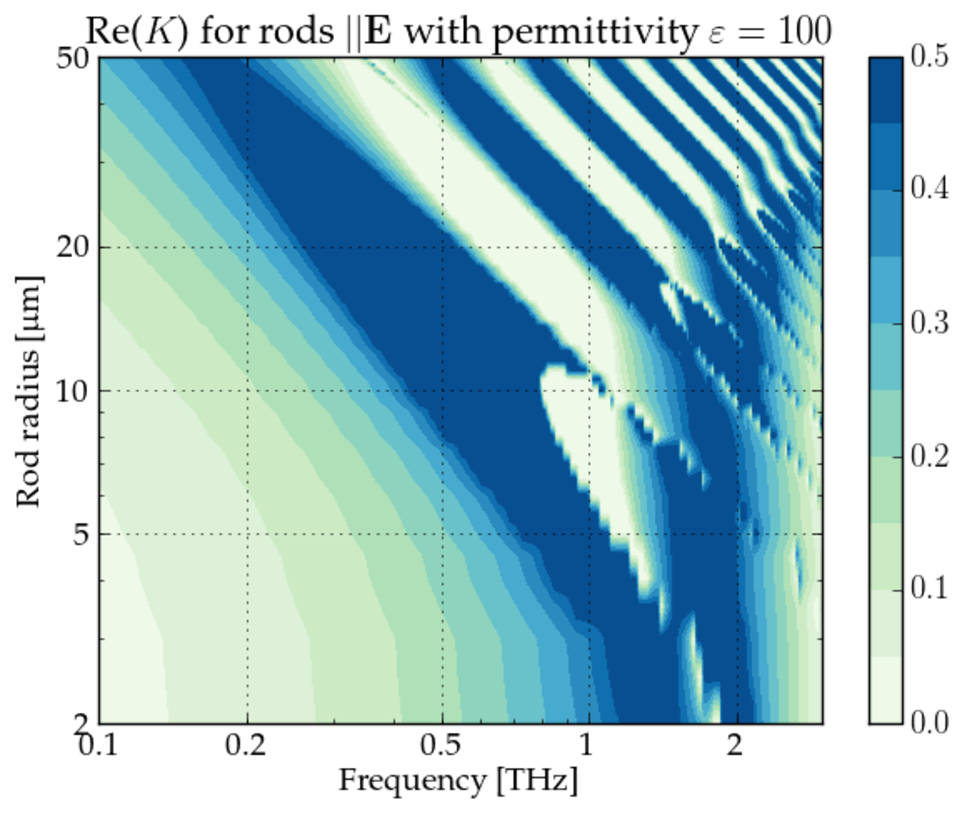
\includegraphics[width=8cm]{img/old/ERods_eps100_radiusscan.pdf}
\end{figure}


\begin{figure}[ht] \caption{Experimental and numerical data for strontium titanate bars $||\mathbf E$ of rectangular cross-section $26 \times 66\;\upmu$m. }\label{fg_ebars_exp} \centering 
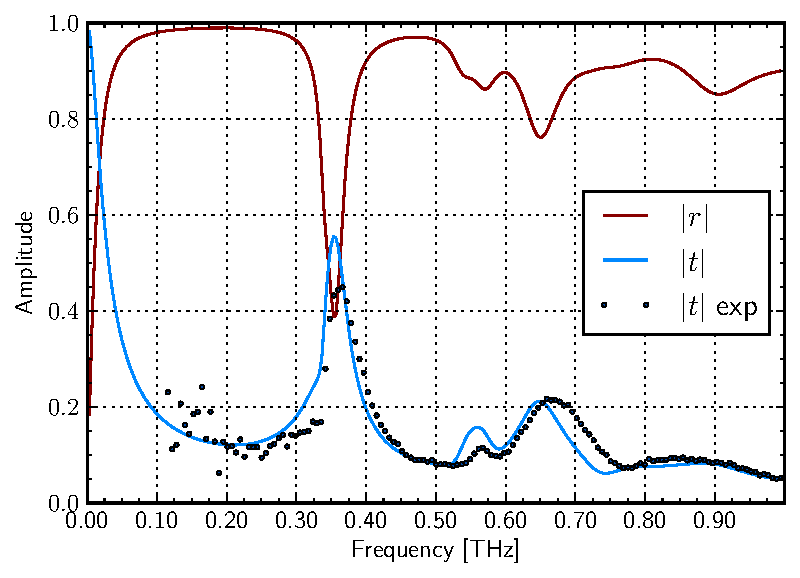
\includegraphics[width=11cm]{img/STObar_rt.pdf} 
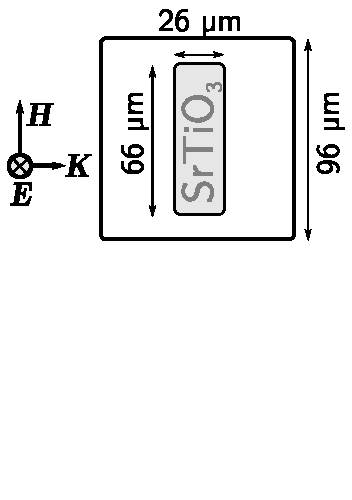
\includegraphics[width=4cm]{img/EBars_STO_sketch.pdf}
\end{figure}
% XRectWire_resolution=2.00e-06_comment=STO_simtime=1.50e-10_yspacing=9.60e-05_epsilon=6.00e+02_cells=1.00e+00_padding=5.00e-05_width=6.40e-05_monzd=1.00e-04_thick=2.60e-05_Kx=0.00e+00_Ky=0.00e+00
The dielectric bars parallel to the electric field represent the same structure as previously discussed, except that it is orthogonally rotated. There is however a qualitative difference in that the high-permittivity dielectric is continuous along the direction of the electric field, so the effect of the dielectric is expected to be much stronger. This results in that the first Mie resonance is the \textit{electric} one. Its overlap with the next magnetic resonance can eventually lead to negative index of refraction in such a structure \cite{peng2007, vynck2009}. If the permittivity of the rods is chosen to be $\varepsilon = 100$ and the periodicity of the lattice $a = 100\;\upmu$m, the negative index of refraction occurs in a narrow range of radii from 9 to 12 $\upmu$m. The behaviour of this structure with the desired radius is depicted in Fig. \ref{fg_erod_radius11}a,b.

In order to form a photonic band with a negative index of refraction, both the permittivity and permeability need to be negative. In the structure discussed, this is made possible by the frequencies of the electric and magnetic Mie resonances being close enough to overlap.
The electric resonance would be surrounded by its broad band gap between the frequencies spanning from $0.13 \cdot\frac{c}{100\;\upmu\text{m}} \approx 400$ GHz to  $0.38 \cdot\frac{c}{100\;\upmu\text{m}} \approx 1140$ GHz. This is also confirmed by Fig. \ref{fg_erod_radius11}a where the mode shapes X1 and $\Gamma$4 perfectly correspond to the electric Mie resonance. 

For the interesting range of radii around 11 $\upmu$m, the magnetic resonance introduces a new, narrow photonic band starting from X2. Now, moving on to the right plot of Fig. \ref{fg_erod_radius11}b, we can clearly identify the resonant frequencies of 815 and 900 GHz. They cause abrupt skips of the refractive index which always shift the index of refraction by one Brillouin zone down.\footnote{The individual resonance appears to be the only mechanism that causes $N'_{\text{eff}}$ to \textit{decrease} in the spectrum. In photonic bands, no matter if $N_{\text{eff}} > 0$  or $N_{\text{eff}} < 0$, the real part of $N_{\text{eff}}$ always grows in accordance with the Foster theorem. This is confirmed by the FDTD results and by their compliance to Kramers-Kronig relations. To illustrate this, the Hilbert transform of the refractive index is plot as the thin pink line and it nearly perfectly follows the green curve over whole spectrum, except for an additive constant. There is  only one acceptable physical solution that is compatible with the Kramers-Kronig relations.}
The resonance is accompanied by a sharp peak in the imaginary part of refractive index $N''$ and by transmission amplitude touching zero ($|t| = 0$). As both Mie resonances precede the Bragg gap, the index of refraction is pushed into negative values and the following photonic band gap $N' < 0$.

For completeness we add the FDTD results with effective permittivity and permeability, computed for the entire spectrum. These quantities however seem to have a useful physical interpretation only within the photonic bands, or within those parts of the photonic band gaps where $N = 0$. 
\\

The dispersion curves of the rods with radii different than 11 $\upmu$m are compared in Fig. \ref{fg_ebar_radiusscan}b based on multiple FDTD simulations. The individual resonances are again easy to be distinguished by abrupt changes from white to blue or vice versa (i.e. skips between the Brillouin zones). We can see that for radii below 8 $\upmu$m the magnetic resonance is at too high frequencies, forming its separate band gap. For even thinner rods at the very bottom edge of the plot, no individual resonance intersects with the first Bragg  band gap at all. 

An interesting qualitative change of the structure response occurs when the rods get slightly thicker than discussed above, say $r > 12\;\upmu$m. The electric and magnetic resonance frequencies do never cross over, but instead they  and an ordinary Bragg band gap remains. The transmission curve of single cell (Fig. \ref{fg_erod_radius11}) continuously shifts up and does not touch zero anymore. We may conclude that for rod radius being too high, the structure no more exhibits the negative index of refraction and starts to behave similar to the 1-D photonic crystal discussed above.
% TODO explanation by nodal planes

%The dependence of the folded wavenumber $\text{Re}(K)$ for high-permittivity rods $||\mathbf E$ is plot in Fig. \ref{fg_ebar_radiusscan}b. Starting from very thin rods ($r=2$ \um) at the very bottom of the plot, we can see the first band gap (1.3 to 1.5 THz) denoted by darkest blue is purely of the Bragg type, followed by a 

Comparing the low-permittivity and high-permittivity cases in Fig. \ref{fg_ebar_radiusscan}a,b, one can see there exists some minimum limit for the permittivity contrast that is necessary for both electric and magnetic resonances to be located in the first gap simultaneously. We determined this scale-invariant value to be roughly 80.

As a little verification that the numerical computations give sound results, we attach experimental transmission measurement of the rod array in Fig. \ref{fg_ebars_exp}.
The bars used had rectangular cross-section, being 26 $\upmu$m thick, 66 $\upmu$m  wide and their periodicity along the $y$-axis was 96 $\upmu$m.  The experimental data (points) are compared to FDTD simulation data of an identical structure (lines). The material used was strontium titanate, best matched by simulation where the permittivity was set to $\varepsilon^{\text{(1 THz)}} = 365 + 62i$.  While this structure can not provide the negative index of refraction and has very high losses, it can act as a temperature-tunable filter. The transmission peaks can be clearly identified with resonant modes and it was observed that the frequencies of the modes shift with different slope depending on parameters.  
} 
%}}}

\add{ %{{{ FROM OPEX
\begin{figure}
\centering 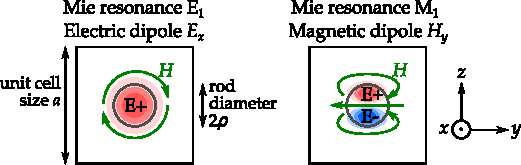
\includegraphics[width=14cm]{img/ERods_1st_and_2nd_Mie_resonance.pdf}
\caption{(a) Perspective view of the unit cell\add{; (b) its}
cross-sections with the resonant modes excited by a plane wave with $\mathbf{E}||x,
\mathbf{H}||y$ and $\mathbf{k}||z$. The first Mie resonance has an electric dipole moment
only, while the second one has a magnetic dipole moment instead. The red and blue color
shows positive and negative values of the $E_x$ component of the electric field, while the magnetic field is
represented by the arrows. }\label{fg_sketchfield}
\end{figure}

Our structure \add{(see Fig.\ref{fg_sketchfield}a)} is defined by a square unit 
cell with the linear dimension $a$ periodically
distributed in the $yz$ plane; the dielectric rod parallel to $x$-axis with 
radius $\rho$
and permittivity $\varepsilon_r$ is positioned in its center. We employed the
finite-difference time-domain (FDTD) simulation package MEEP 
\cite{oskooi2010meep} to
obtain the scattering coefficients (complex reflectance $r$ and transmittance 
$t$) of a
structure with variable number of unit cells along the wave vector direction 
$k\parallel
z$. The incident wave is polarized $E\parallel x$, periodic boundary conditions 
were
applied in the $y$-direction. We performed the 
simulations for a single layer ($y$-periodic boundary conditions 
only). Its effective properties are almost identical to those of the
corresponding multilayer structure. We checked that for this geometry, 
the retrieved effective
parameters depend only negligibly on the number of unit cells in the 
$z$-direction. The relevance of the calculations with a single layer was 
further confirmed by current-driven homogenization simulations \cite{Markel13} in several particular cases (same geometries as in 
Fig.~\ref{fg_spec}) which yielded a response in a very good agreement 
with the FDTD results.
The effective parameters were \add{then} retrieved from complex
transmittance and reflectance spectra \cite{smith2002determination}. 
\add{Alternative means of obtaining the effective parameters are discussed in 
	Ref. \cite{Simovski09}. When 
	inverting the Fresnel-Airy formulas, the correct solutions have to be chosen 
	in the different parts of the $\Neff(\omega)$, $\Zeff(\omega)$ spectra
\cite{Simovski09}; to this aim, Kramers-Kronig relations as well as the 
conditions of a passive medium Im$(\Neff)>0$ and Re$(\Zeff)>0$ were used.} 

The retrieved value of the complex effective index of refraction $\Neff(f)$ 
defines the
magnitude of the wave vector
\begin{equation}\label{eq_wave_vector}
k(f) = 2\pi f \Neff(f) /c\,.
\end{equation}
Note that the retrieval procedure  implies that 
the wave vector
introduced by Eq. (\ref{eq_wave_vector}) is defined in an unfolded reciprocal 
space. 

A Bragg resonance occurs when an integer number of half-wavelengths fit into one 
unit cell, i.e.,  when
\begin{equation}\label{eq_BZ}
k(f) = \frac{q \pi}{a}\,,
\end{equation}
where $q$ is a non-zero integer. In such a situation, the wave vector is located at a
Brillouin zone boundary. The purely real values of $k$ then describe photonic band edges.
In a band edge state, a standing wave appears in the structure and it is characterized by
exactly $q$ nodal planes dividing each unit cell in the transverse direction to $q+1$
disconnected parts. The band edges delimit a photonic {\itshape Bragg band gap} where
only evanescent waves described by $\Neff''>0$ can exist.
We can write an equation analogous to (\ref{eq_BZ}) for the real part of the refractive
index:
\begin{equation}\label{eq_BZN}
\Neff'(f) = \frac{q c}{2 a f}\,;
\end{equation}
its hyperbolic behavior versus frequency reflects the pinning of the wave vector to the
Brillouin zone boundary inside the Bragg band gap.

Another case of interest where evanescent waves are obtained is that of $\Neff' = 0$
(center of the first Brillouin zone, $q=0$) and $\Neff''>0$. Here the waves exponentially
decay in the medium without any phase change. However, this behavior has a different
origin: it is connected to a plasma-like response of the material ($\varepsilon<0$ or
$\mu<0$) and in this paper we use the term \textit{plasma band gap} to refer to it.

The Kramers-Kronig relations require that for any structure studied, $\Neff'(f)$ [or,
equivalently, $k(f)$] attains and finally crosses the Brillouin-zone boundaries when the
frequency is sufficiently increased. While usually the convention is used that the
corresponding curves are folded back into the first Brillouin zone, in this paper we plot
$\Neff'(f)$ in the original (unfolded) Brillouin zones resulting from the retrieval
algorithm. This can be clearly observed on the dispersion of the refractive index in
Fig.\ \ref{fg_spec}. In this way we retain the information about the number of the nodal
planes intersecting the unit cell, which is important for our discussion.

\section{Results}
\begin{figure} \centering
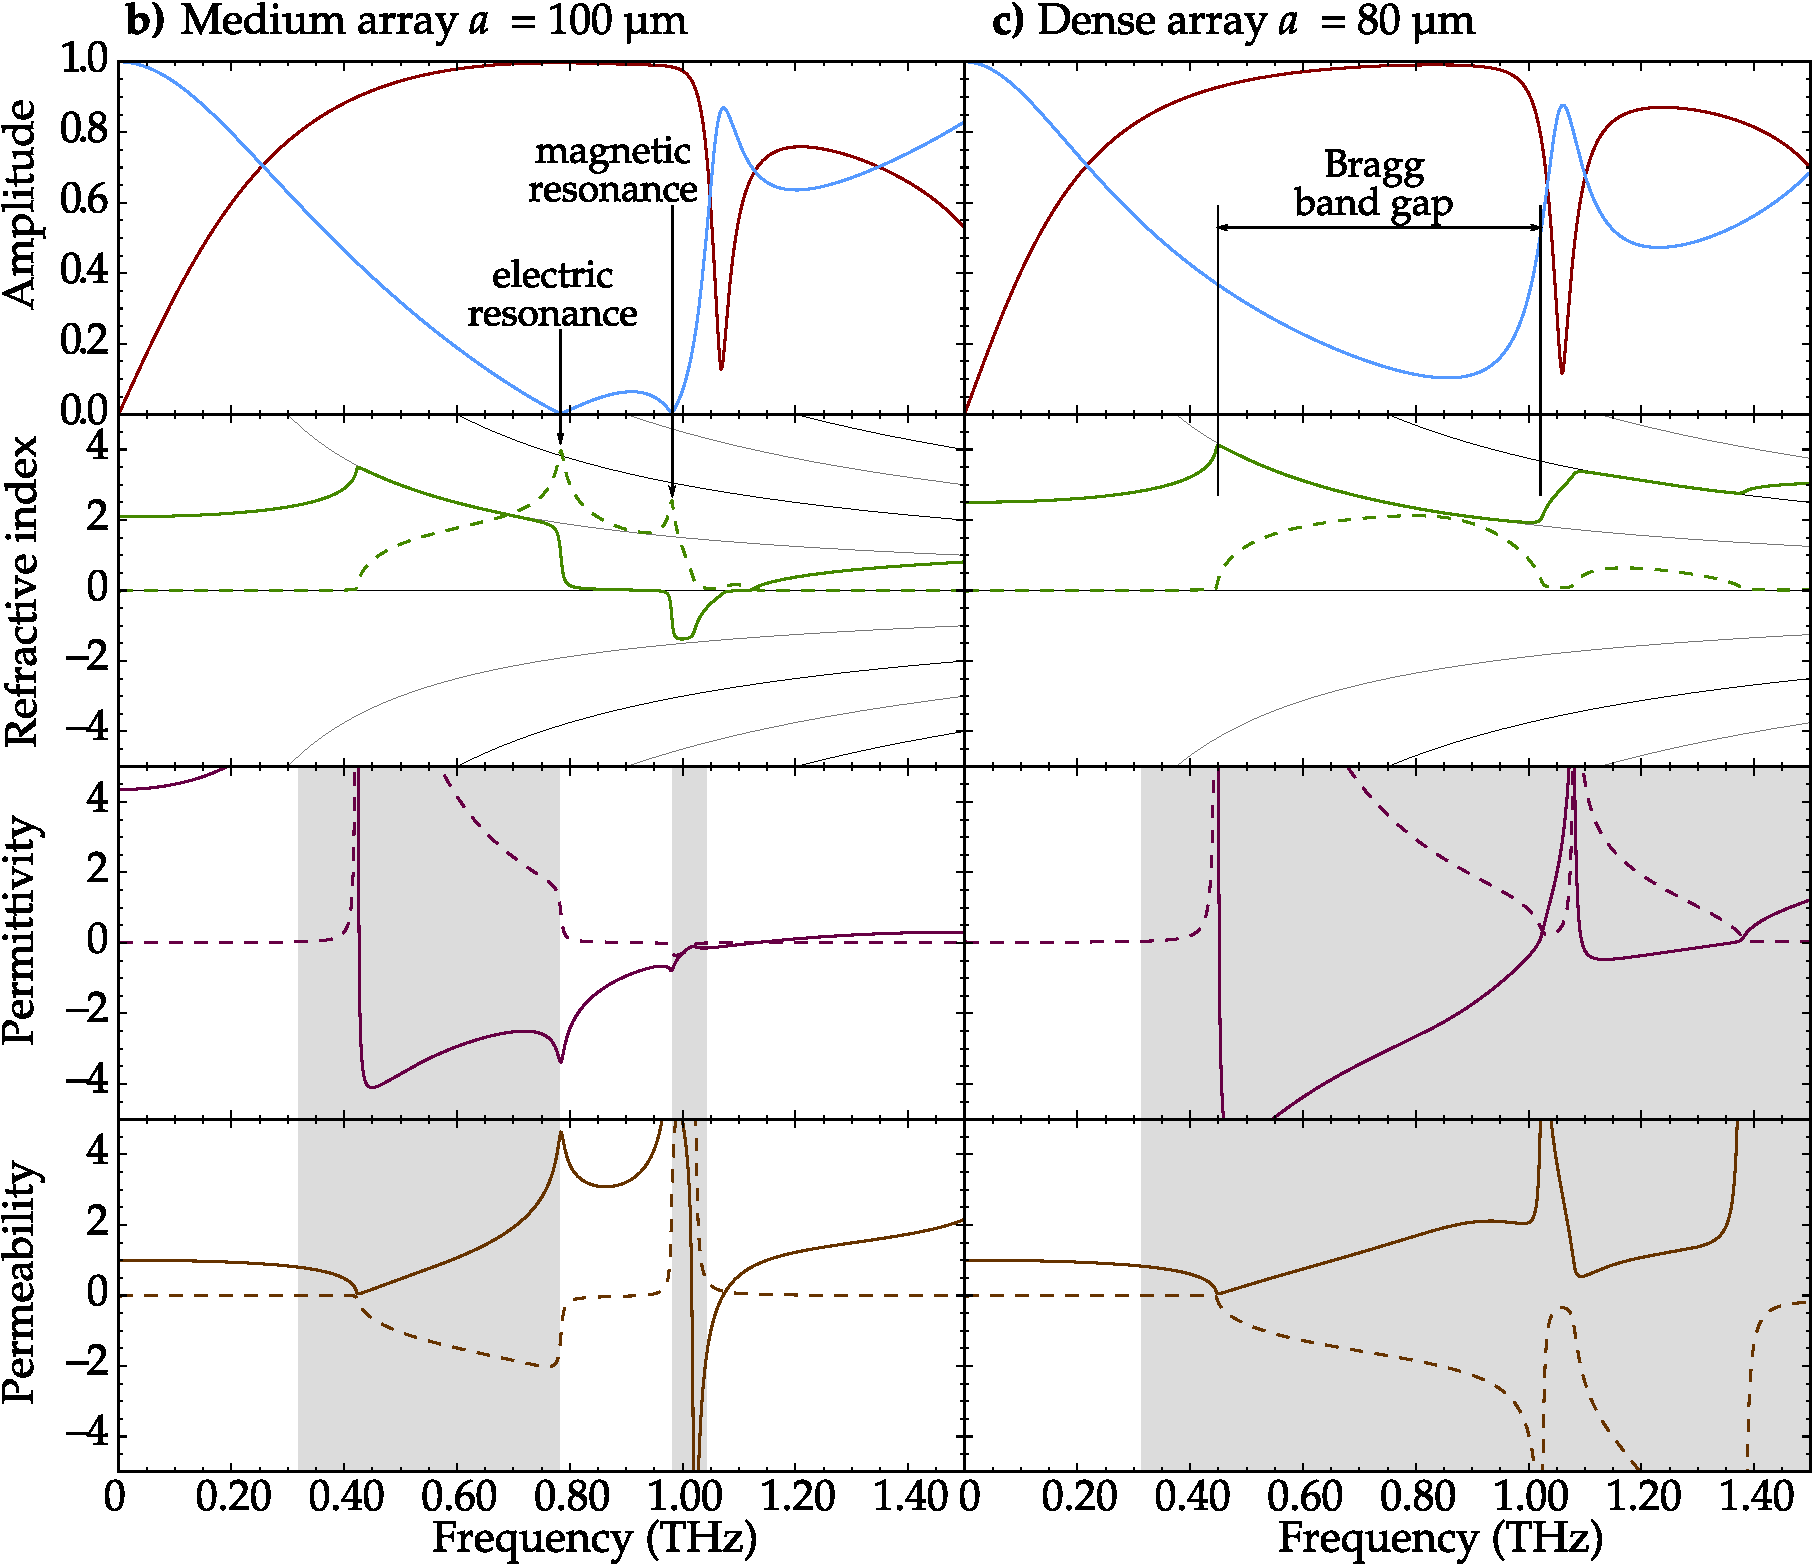
\includegraphics[angle=270,width=105mm]{img/ERods_eps100_double_a100a080_FDTD.pdf}
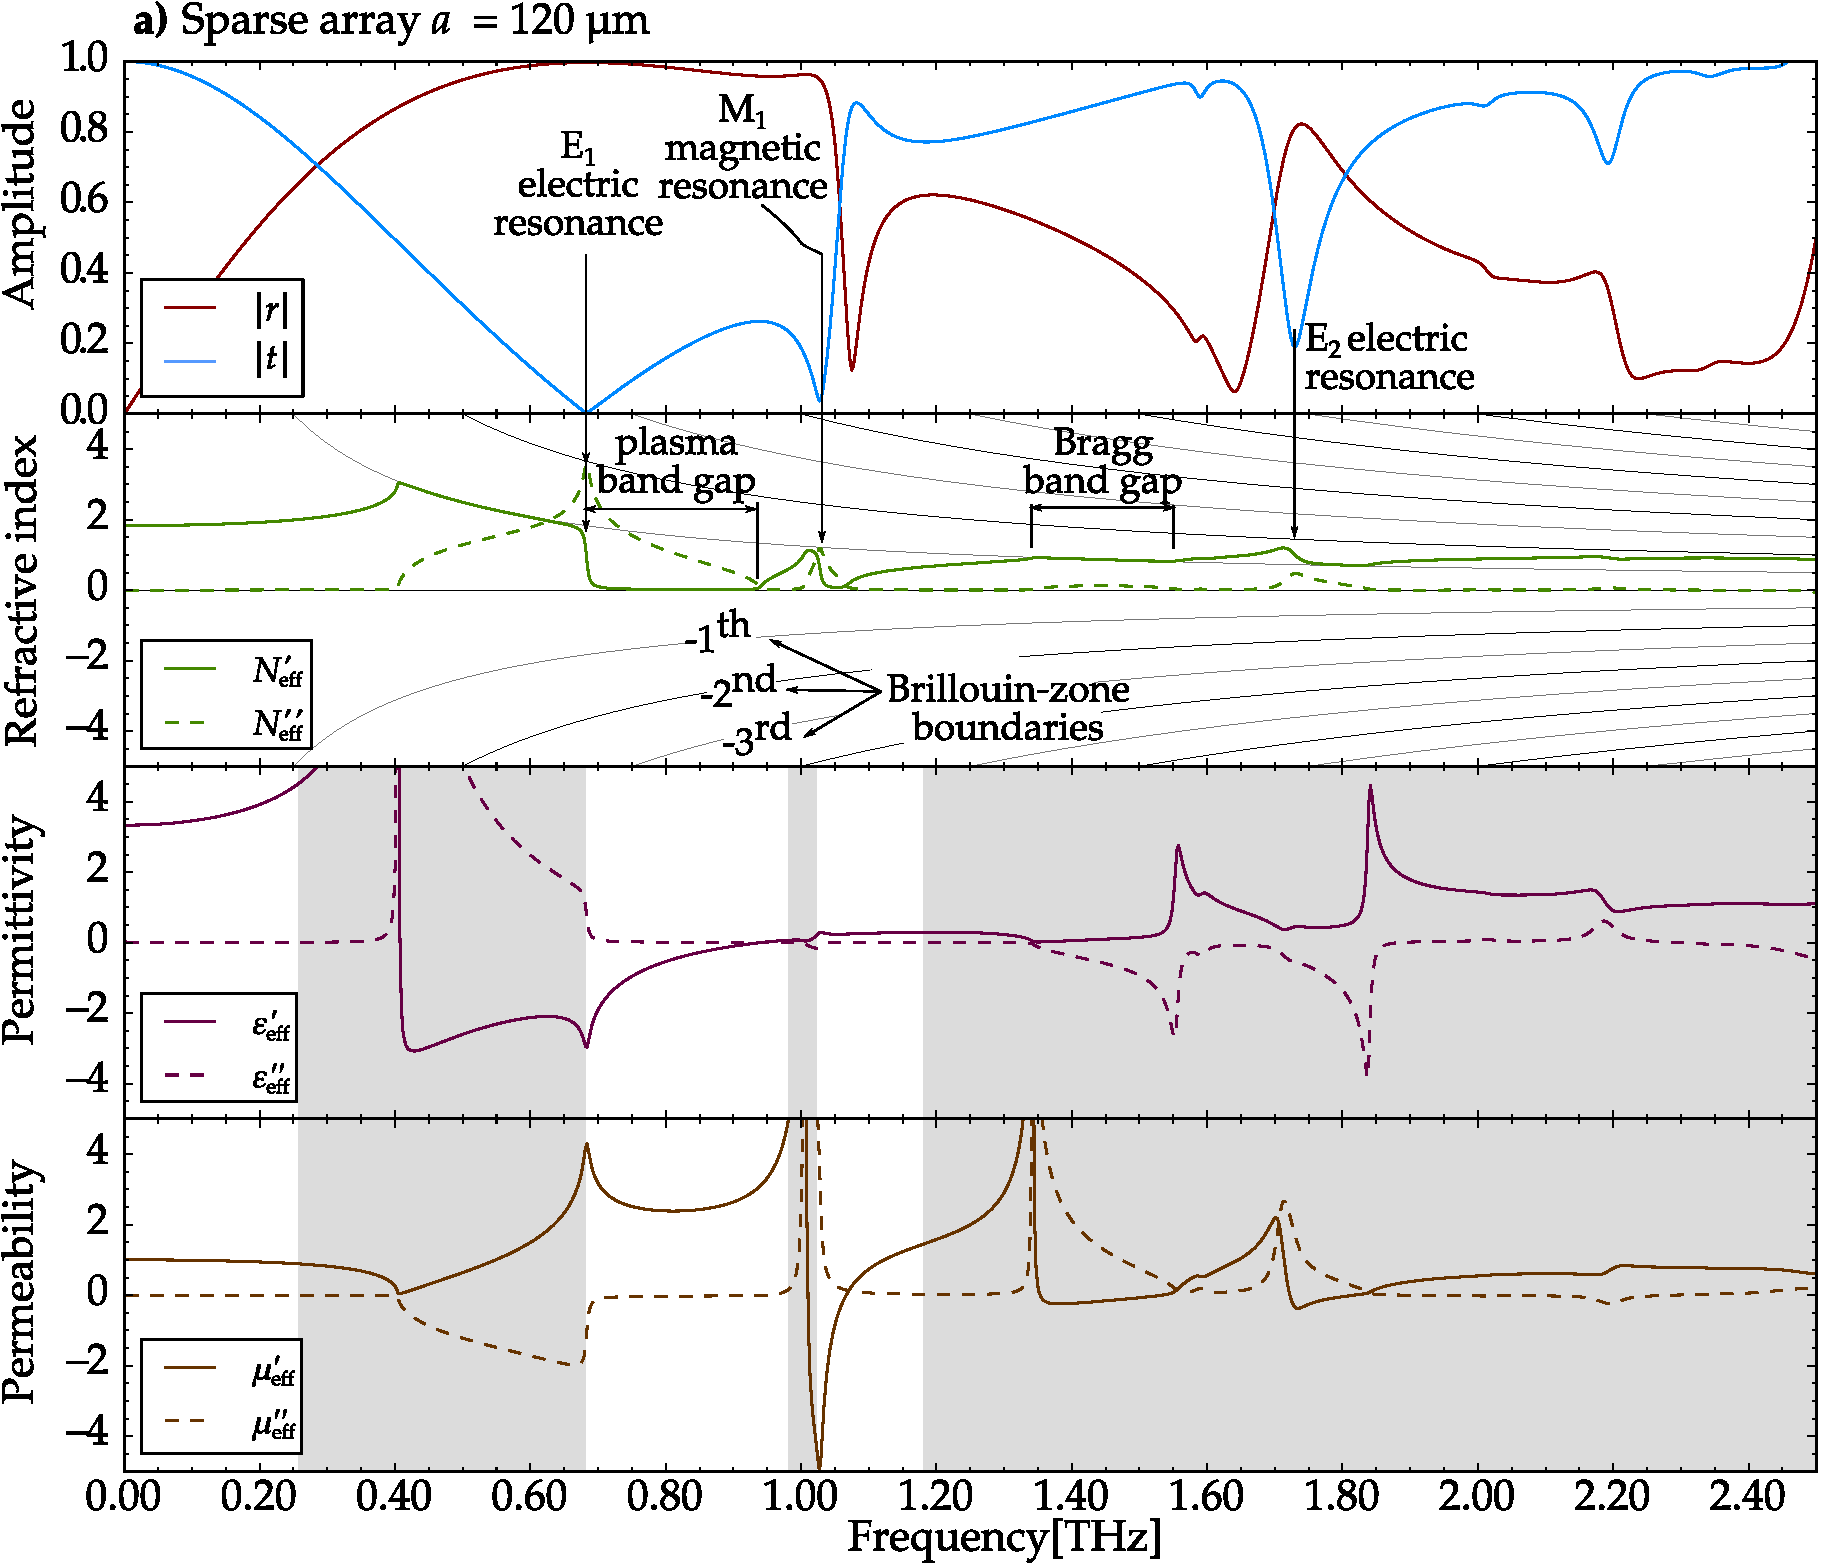
\includegraphics[angle=270,width=105mm]{img/ERods_eps100_single_a120_FDTD.pdf}
\caption{Results of the FDTD simulations for a single layer of dielectric rods with $\varepsilon_{\rm r}= 100$,
$\rho=10$\,$\upmu$m. The spectra of reflection $|r|$ and transmission $|t|$ amplitudes share
their frequency axes with the retrieved complex effective index of refraction $\Neff$,
permittivity $\eeff$ and permeability $\meff$, whose imaginary parts are denoted by
dashed lines. The frequency ranges where $\eeff$ and $\meff$ have no physical
interpretation (Bragg band gaps or higher order photonic bands) are gray shaded.  } \label{fg_spec}
\end{figure}

In the following, we first describe in detail three characteristic cases: we compare the
effective parameters computed for three slightly different unit-cell sizes while the rod
radius and the dielectric permittivity are fixed. The comparison of these cases reveals quite
remarkable changes in the optical behavior of the structure. We then complement this
comparison by a continuous scan of the unit-cell sizes in order to obtain an overview of
all possible types of the response for the rod-based geometry.

In Fig.~\ref{fg_spec}, we show the calculated reflectance and transmittance amplitude
spectra, as well as the effective parameters of three representative structures which
have the same rod radii $\rho = 10$~$\upmu$m, but they differ by the unit-cell size $a =$ 120, 100 and 80 $\upmu$m. These
values of $a$ were selected to illustrate three qualitatively different regimes of
behavior.
The dielectric was defined by a simple lossy model with one high-frequency oscillator, its  permittivity was $\varepsilon_r = 100.1 + 0.5\mathrm{i}$ at 500 GHz.

\paragraph{Sparse array}
In Fig.~\ref{fg_spec}(a), where the unit-cell size $a=120$~$\upmu$m, we can see 
two well separated Mie resonances: the electric one at 680 GHz and the magnetic 
one at 1030 GHz.  The field distribution of the corresponding modes is sketched 
in Fig.~\ref{fg_sketchfield}. The resonance frequencies can be easily identified 
by an abrupt drop in the real part of the effective index of refraction 
$\Neff'$, accompanied by a sharp peak in its imaginary part $\Neff''$. The Mie 
resonances in periodic media without losses must always be adjacent to a Bragg 
band gap. For instance, in Fig.~\ref{fg_spec}(a) at frequencies below the first 
Bragg gap, the electric dipoles within each rod are directed along the electric 
field in the rest of the unit cell. The rods thus positively contribute to the 
refractive index $\Neff'$ which progressively grows until it reaches the first 
Brillouin zone boundary. At this point, the Bragg condition for a photonic 
band-gap is fulfilled and each unit cell is intersected by one nodal plane. This 
is reflected by the dispersion of $\Neff'(f)$ which follows the first 
Brillouin-zone boundary in the first Bragg band gap between 400 and 680\,GHz 
[equivalent to $q=1$ in Eq. (\ref{eq_BZN})]: $$	\Neff'(f) = \frac{c}{2af}\,. $$ 
At 680\,GHz, the electric Mie resonance occurs which dramatically changes the 
near-field photonic properties of the structure. The observed drop in 
$\Neff'(f)$ and the slope change in $\Neff''(f)$ mark the plasma-like character 
of the adjacent part of the band gap which extends up to the plasma frequency of 
the Mie resonance (940\,GHz). In this frequency range the electric dipoles in 
the rods change their direction and induce an electric field opposite to the 
incident one.

For this sparse array of dielectric rods, the first magnetic Mie resonance lies 
at 1030\,GHz, above the plasma frequency of the electric mode.  The second Bragg 
band-gap opens at 1010 GHz and, due to the Mie resonance, it is transformed to a 
plasma band gap at 1030 GHz. The next allowed photonic band starts above 
magnetic plasma frequencies at 1070 GHz. Therefore we observe a very analogous 
behavior near the magnetic resonance. 

For completeness we note that at 1350 GHz, a third Bragg band gap
starts which, unlike the lower-frequency ones, does not contain any Mie resonances 
[see Fig.\ \ref{fg_spec}(a)].

The resonances in the effective permittivity $\eeff=\Neff/\Zeff$ and permeability $\meff
= \Neff\cdot \Zeff$ of a periodic array obviously exhibit shapes very different from the
well-known resonance curves of a damped oscillator\cite{koschny2003resonant}. In the two
separate plasma band gaps we obtain either $\eeff < 0$ or $\meff<0$, i.e. the usual
behavior observed in the reststrahlen bands of resonances. However, in the Bragg band
gaps occurring just below these spectral ranges the behavior of $\eeff$ and $\meff$ does
not have any useful physical interpretation and it can be understood as a purely formal
frequency dependence: we shaded these ranges with light gray in Fig.~\ref{fg_spec}.

\paragraph{Medium array}
When the unit cell size is reduced to $a=100$~$\upmu$m, as depicted in
Fig.~\ref{fg_spec}(b), the Mie resonances shift slightly. Interestingly, in comparison with the sparse array, the electric
resonance frequency increases from 680 to 780 GHz, and that of the
magnetic resonance decreases from 1030 to 980 GHz. This can be explained by the
inter-cell coupling: the circulating magnetic field of the first resonance is compressed
when the rods get closer, whereas the magnetic dipoles of the second resonance can couple
more easily to each other in the same situation (see Fig.~\ref{fg_sketchfield}).

The converging of the resonance frequencies is linked to the most important
qualitative change in the spectra: the fact that the magnetic resonance occurs at a
frequency where $\eeff'<0$. The first band gap (the lowest continuous frequency region where
$\Neff''>0$) is thus composed of three adjacent regimes: the first Bragg band gap
(425--780 GHz), a plasma band gap (780--980 GHz) and the second Bragg band gap (980--1020
GHz). Every Mie resonance introduces a drop in $\Neff'$, so the following photonic band
(1020--1070 GHz) features a negative index of refraction ($\Neff'<0; \Neff''\approx 0$),
i.e., the phase and group velocities are opposite to each other. We conjecture that the presence of two
Mie resonances in the \textit{first} combined band gap is a necessary and sufficient condition for
$\Neff'<0$ to occur.

Note that the transmittance amplitude reaches quite small values between the Mie
resonances when they are sufficiently close to each other [Fig. \ref{fg_spec}(b)]. This range forms a
well-defined band with a reflectance-to-transmittance contrast much better than that
observed in a planar Fabry-Perot resonator. One layer of dielectric rods with proper
parameters can therefore be applied as a thin, yet very effective filter.

\paragraph{Dense array}
Perhaps an even more surprising change occurs when the rod spacing is further reduced. The Mie resonances get even closer in the
spectrum and eventually they vanish for $a=80$~$\upmu$m [see Fig.~\ref{fg_spec}(c)]. The band gap remains at nearly the same spectral
position as in panel (b) of this figure, but, unlike for the medium array, the value of $\Neff'$ does not drop within
the Bragg band gap. In contrast, it is shifted up to the second Brillouin zone boundary
where it meets the second Bragg band gap as clearly seen in panel (c), indicating that
each unit cell is intersected by two nodal planes in this state.

The reason of this behavior is related to the change of the nodal plane topology caused
by the inter-cell coupling. When the rods are far from each other ($a\gtrsim
100$~$\upmu$m), the individual Mie resonances create closed regions delimited by a nodal
surface where the fields are opposite to the rest of the unit cell. Upon reducing the
unit-cell size ($a\lesssim 80$~$\upmu$m), the regions of opposite fields start to overlap
with those from the neighboring cells and the corresponding nodal surfaces interconnect
and open. This pair of open nodal surfaces dividing the unit cell manifests itself by a
qualitative change of the $\Neff'$ spectrum towards a shape typical for one-dimensional
photonic crystals.


The Mie resonances are caused by the field confinement near the high permittivity
elements. They always manifest themselves as sharp peaks in the imaginary part of the
index of refraction ($\Neff''$), and in Fig.~\ref{fg_drawn100} they are denoted by thick
solid curves. Their electric- or magnetic-dipole character is identified by the letters
"E" or "M" above the plot, respectively.

As it can be seen in Figs.~\ref{fg_spacingscan100} and \ref{fg_drawn100}, the pairs
of electric and magnetic Mie resonances form U-shaped curves, at the bottom of which the
resonances come closer in frequency to each other and eventually they disappear when the
unit-cell size $a$ is further reduced. The resonances influence the whole spectra of the
refractive index $\Neff'$, so the position of this U-curve delimits the range of $a$ for
which a photonic band with $\Neff' < 0$ and $\Neff'' \approx 0$ can be found. This
negative-index band is shown in black in Fig.~\ref{fg_drawn100}.

\begin{figure}
	\centering
    \includegraphics[width=7cm]{img/ERods\_eps030\_spacingscan\_drawn\_bands.pdf}
    \caption{Scheme of band gaps and Mie resonances for dielectric permittivity $\varepsilon_r = 30$. The Mie resonances shift to higher frequencies relative to the band gaps and no $\Neff'<0$ region is formed for any unit cell size (cf. Fig. \ref{fg_drawn100})}
\label{fg_drawn030}
\end{figure}

Note that the frequencies of the Mie resonances deviate from their free-space 
values when the rod distance is reduced. In fact, these resonances help to form 
the photonic band gaps (both Bragg and plasma band gaps) due to their 
dispersion. As a consequence, these resonances must be always located inside a 
frequency range with $\Neff''>0$.

\section{Discussion}
Having analyzed the case of high dielectric ($\varepsilon_r=100$) permittivity rods, we
will draw below implications for building a negative-index MM from available dielectrics.
Another series of simulations implies that reducing the dielectric permittivity has the main effect
to shift all the Mie resonances to higher frequencies (also with respect to the photonic
bands). As a result, the band with $\Neff'<0$ gets gradually narrower and, for the rod
permittivity below about 50, we do not find any cell size $a$ that would imply the first
and second Mie resonances in the first photonic band as illustrated for $\varepsilon_r = 30$ in Fig. \ref{fg_drawn030}. This means that the value of
$\varepsilon_{r} \approx 50$ is the minimum for obtaining a negative index of refraction
in any square array of cylindrical rods. Note that one would come to a very similar value
of minimum permittivity for the case of a square array of bars with a slightly different
shape, e.g. a square cross-section. 

A sufficiently high permittivity can be found in the microwave and terahertz ranges, 
in a variety of materials, for example in titanium dioxide with $\varepsilon_r \approx 92$ \cite{nemec2009tunable} 
or in various ferroelectrics like strontium titanate \cite{skoromets2011tuning}. However, practical applications of
the high-permittivity dielectrics in the THz range can be restricted by high dielectric
losses due to low-frequency phonon absorption tails. To our knowledge, there is no
material providing such a high permittivity in the near-infrared or optical ranges. This
eliminates the possibility to build a MM at these frequencies with $\Neff'<0$ based on dielectric
rods.

Finding a valid negative index of refraction $\Neff'$ for a photonic structure implies
that the Snell law can be used to predict the negative refraction at an interface, provided
the iso-frequency contours can be well approximated by a circle. This condition is fulfilled
when the resulting wave vector is oriented close to a symmetry axis of the structure, or when 
the wave vector is negligible compared to the reciprocal lattice vector (i.e. $k\ll \frac{\pi}{a}$ and 
thus $|\Neff'| \ll \frac{c}{2af}$). 
In the latter case the iso-frequency contours of the isotropic structure approach a circular shape
near the $\Gamma$-point in the Brillouin zone center. 
By contrast, the opposite implication is not necessarily applicable---a structure with a high
enough spatial dispersion can still refract under negative angles, 
yet its refractive index computed along a symmetry axis never reaches negative values and the phase difference across each its 
unit cell is positive and can be comparable to $\pi$.
For example, it was suggested earlier  \cite{Vynck2009} that an array of 
silicon rods ($\varepsilon_r \approx 12$) can constitute a true left-handed metamaterial ($\Neff'<0$).
In agreement with the results presented above, we believe that the negative refraction 
is not a sufficient proof of $\Neff'<0$, which would require a much higher permittivity contrast than that of silicon. 
We conclude that the electromagnetic behavior observed previously \cite{Vynck2009} has to be 
described by means of the PhC dispersion curves. 

We demonstrated that for $\Neff'<0$, not only the high permittivity contrast, but also 
a correct geometry is required. A wedge filled
with an array of square-shaped high-dielectric bars was previously reported 
refracting under negative angles \cite{peng2007}. The high filling fraction ($0.44^{2}$)
simultaneously with a permittivity of $\varepsilon_r \approx 600$ clearly qualified this
structure as \textit{dense}. Using the above described approach, we computed its spectra 
qualitatively similar to Fig.~\ref{fg_spec}(c) and no band with $\Neff' < 0$ was resulting from our effective index
retrieval. However, when we reproduced the wedge experiment numerically, our simulations
confirmed that it does refract the light under negative angles.

This structure lies at the boundary between the criteria for MMs and PhCs described in the Introduction.
To determine its refraction angle, in general, it is not possible to use the 
concept of 
 the effective refractive index and
its iso-frequency contours have to be used instead (like in PhCs). At the same 
time, this structure was proved
to partially retain negative refraction even under randomization of the positions
of the dielectric bars \cite{peng2007}, implying that most of the resonant energy is concentrated inside
the dielectric (which is characteristic of MMs).
}
%}}}

\begin{figure} \caption{img/ERods\_eps100\_R11\_PWEM.pdf}  \centering 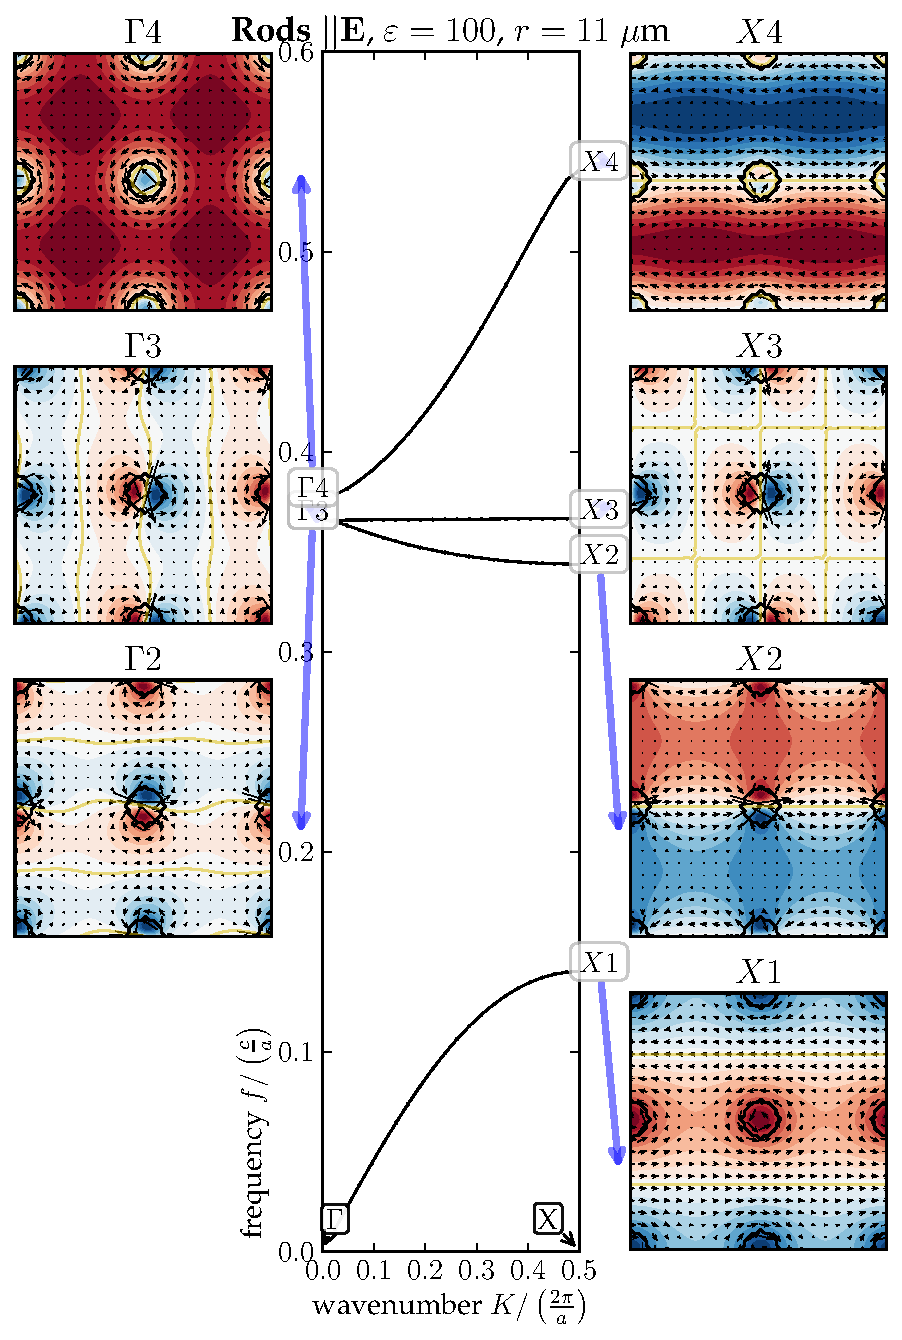
\includegraphics[width=10cm]{img/ERods_eps100_R11_PWEM.pdf} \end{figure} \clearpage
%  \begin{figure} \caption{img/ERods\_eps100\_single\_a120\_FDTD.pdf}  \centering 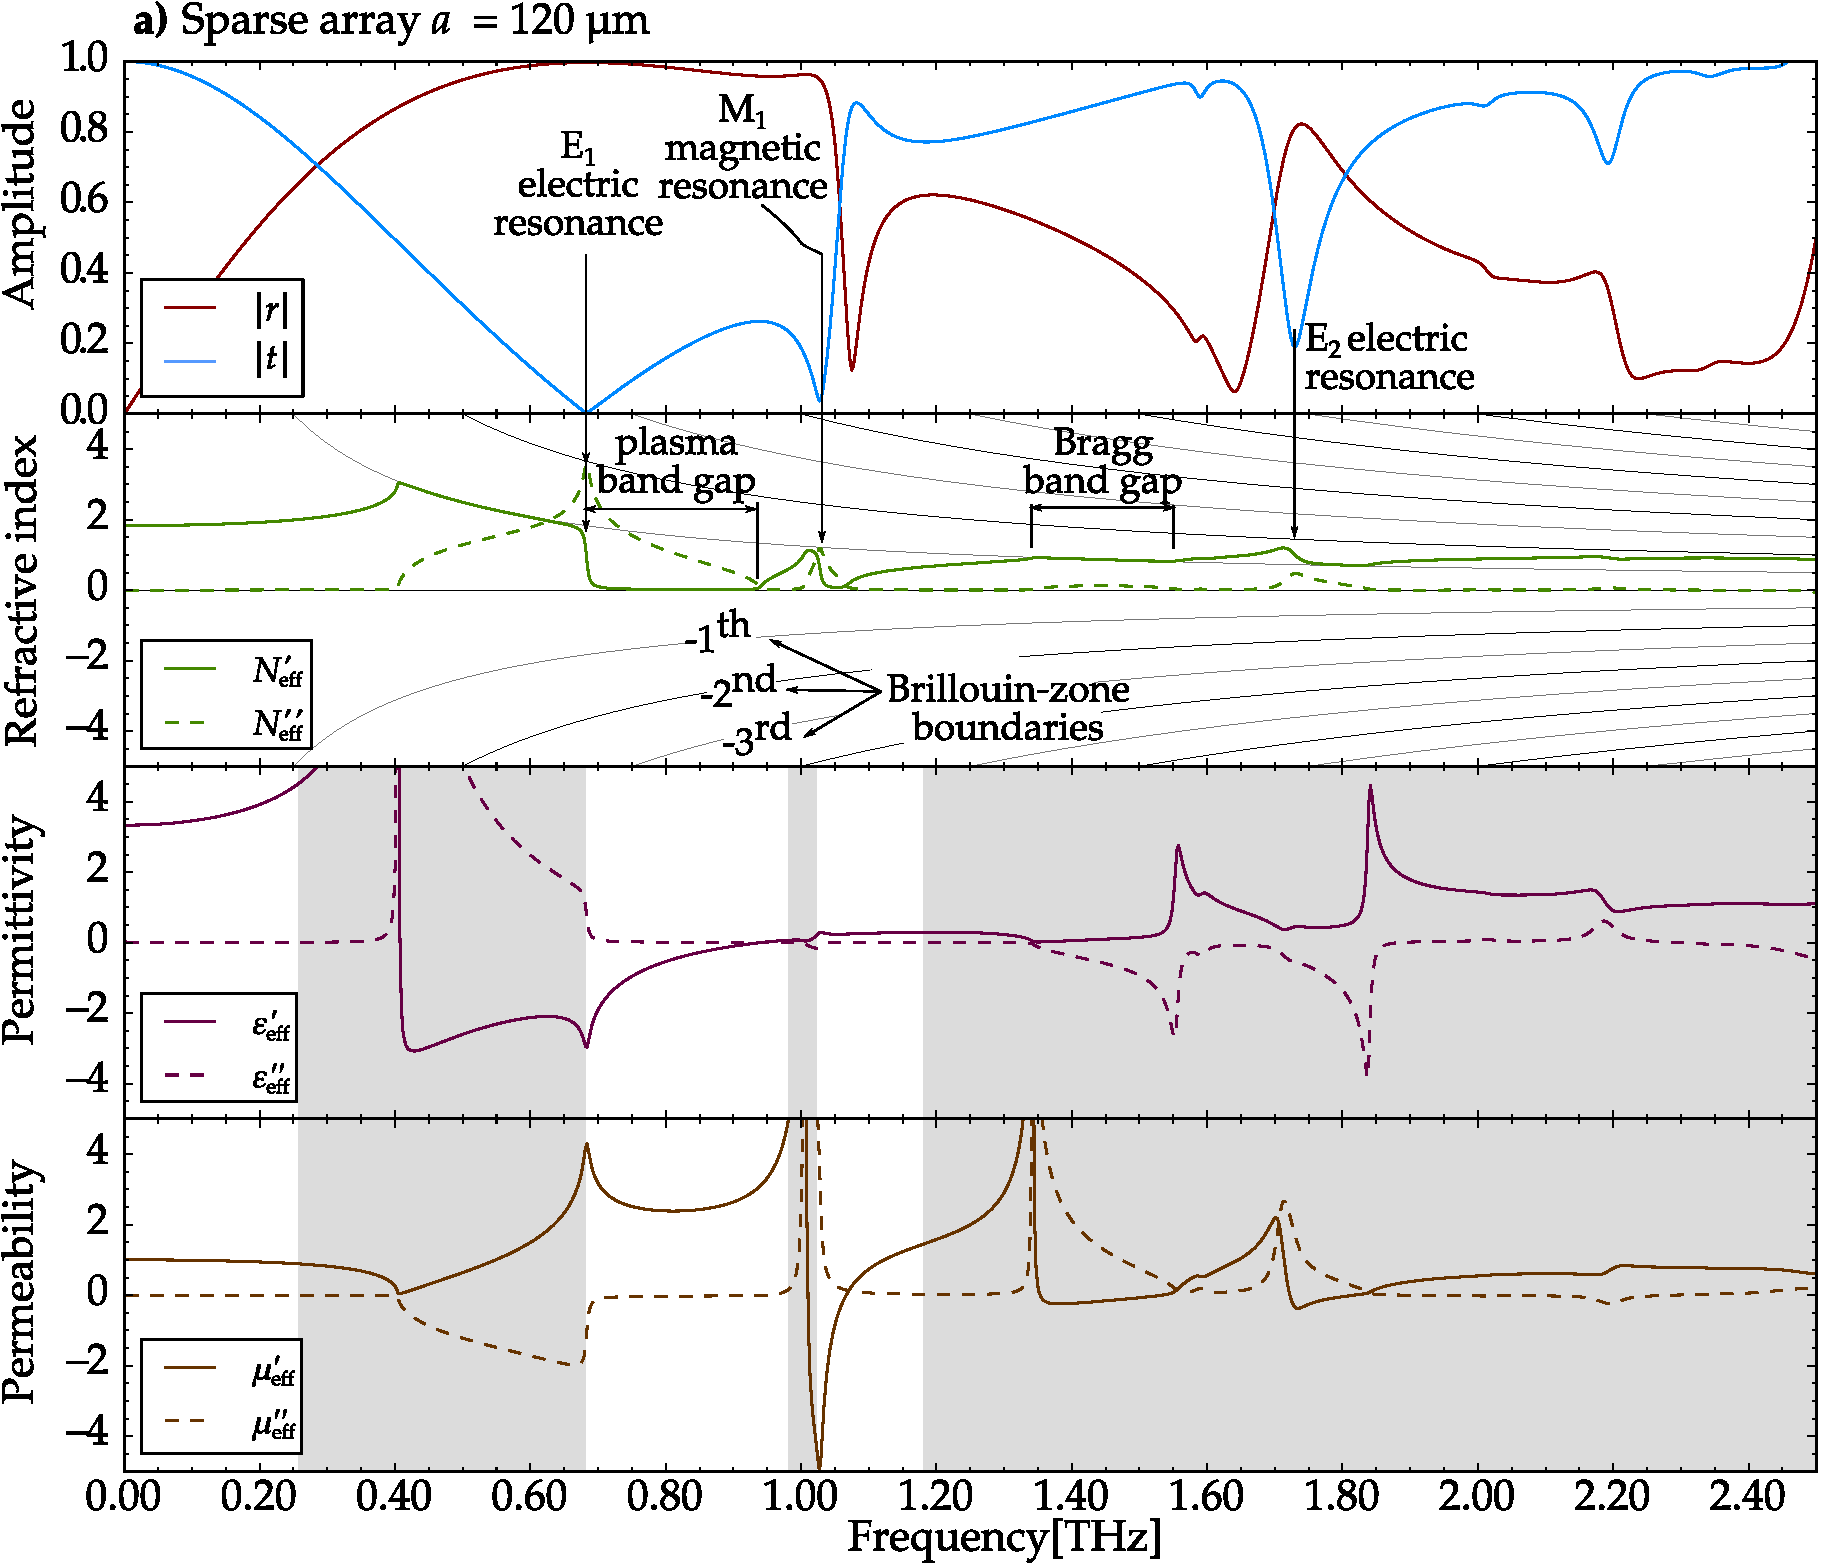
\includegraphics[width=10cm]{img/ERods_eps100_single_a120_FDTD.pdf} \end{figure} \clearpage
%  \begin{figure} \caption{img/ERods\_eps100\_triple\_a150a100a080\_FDTD.pdf}  \centering 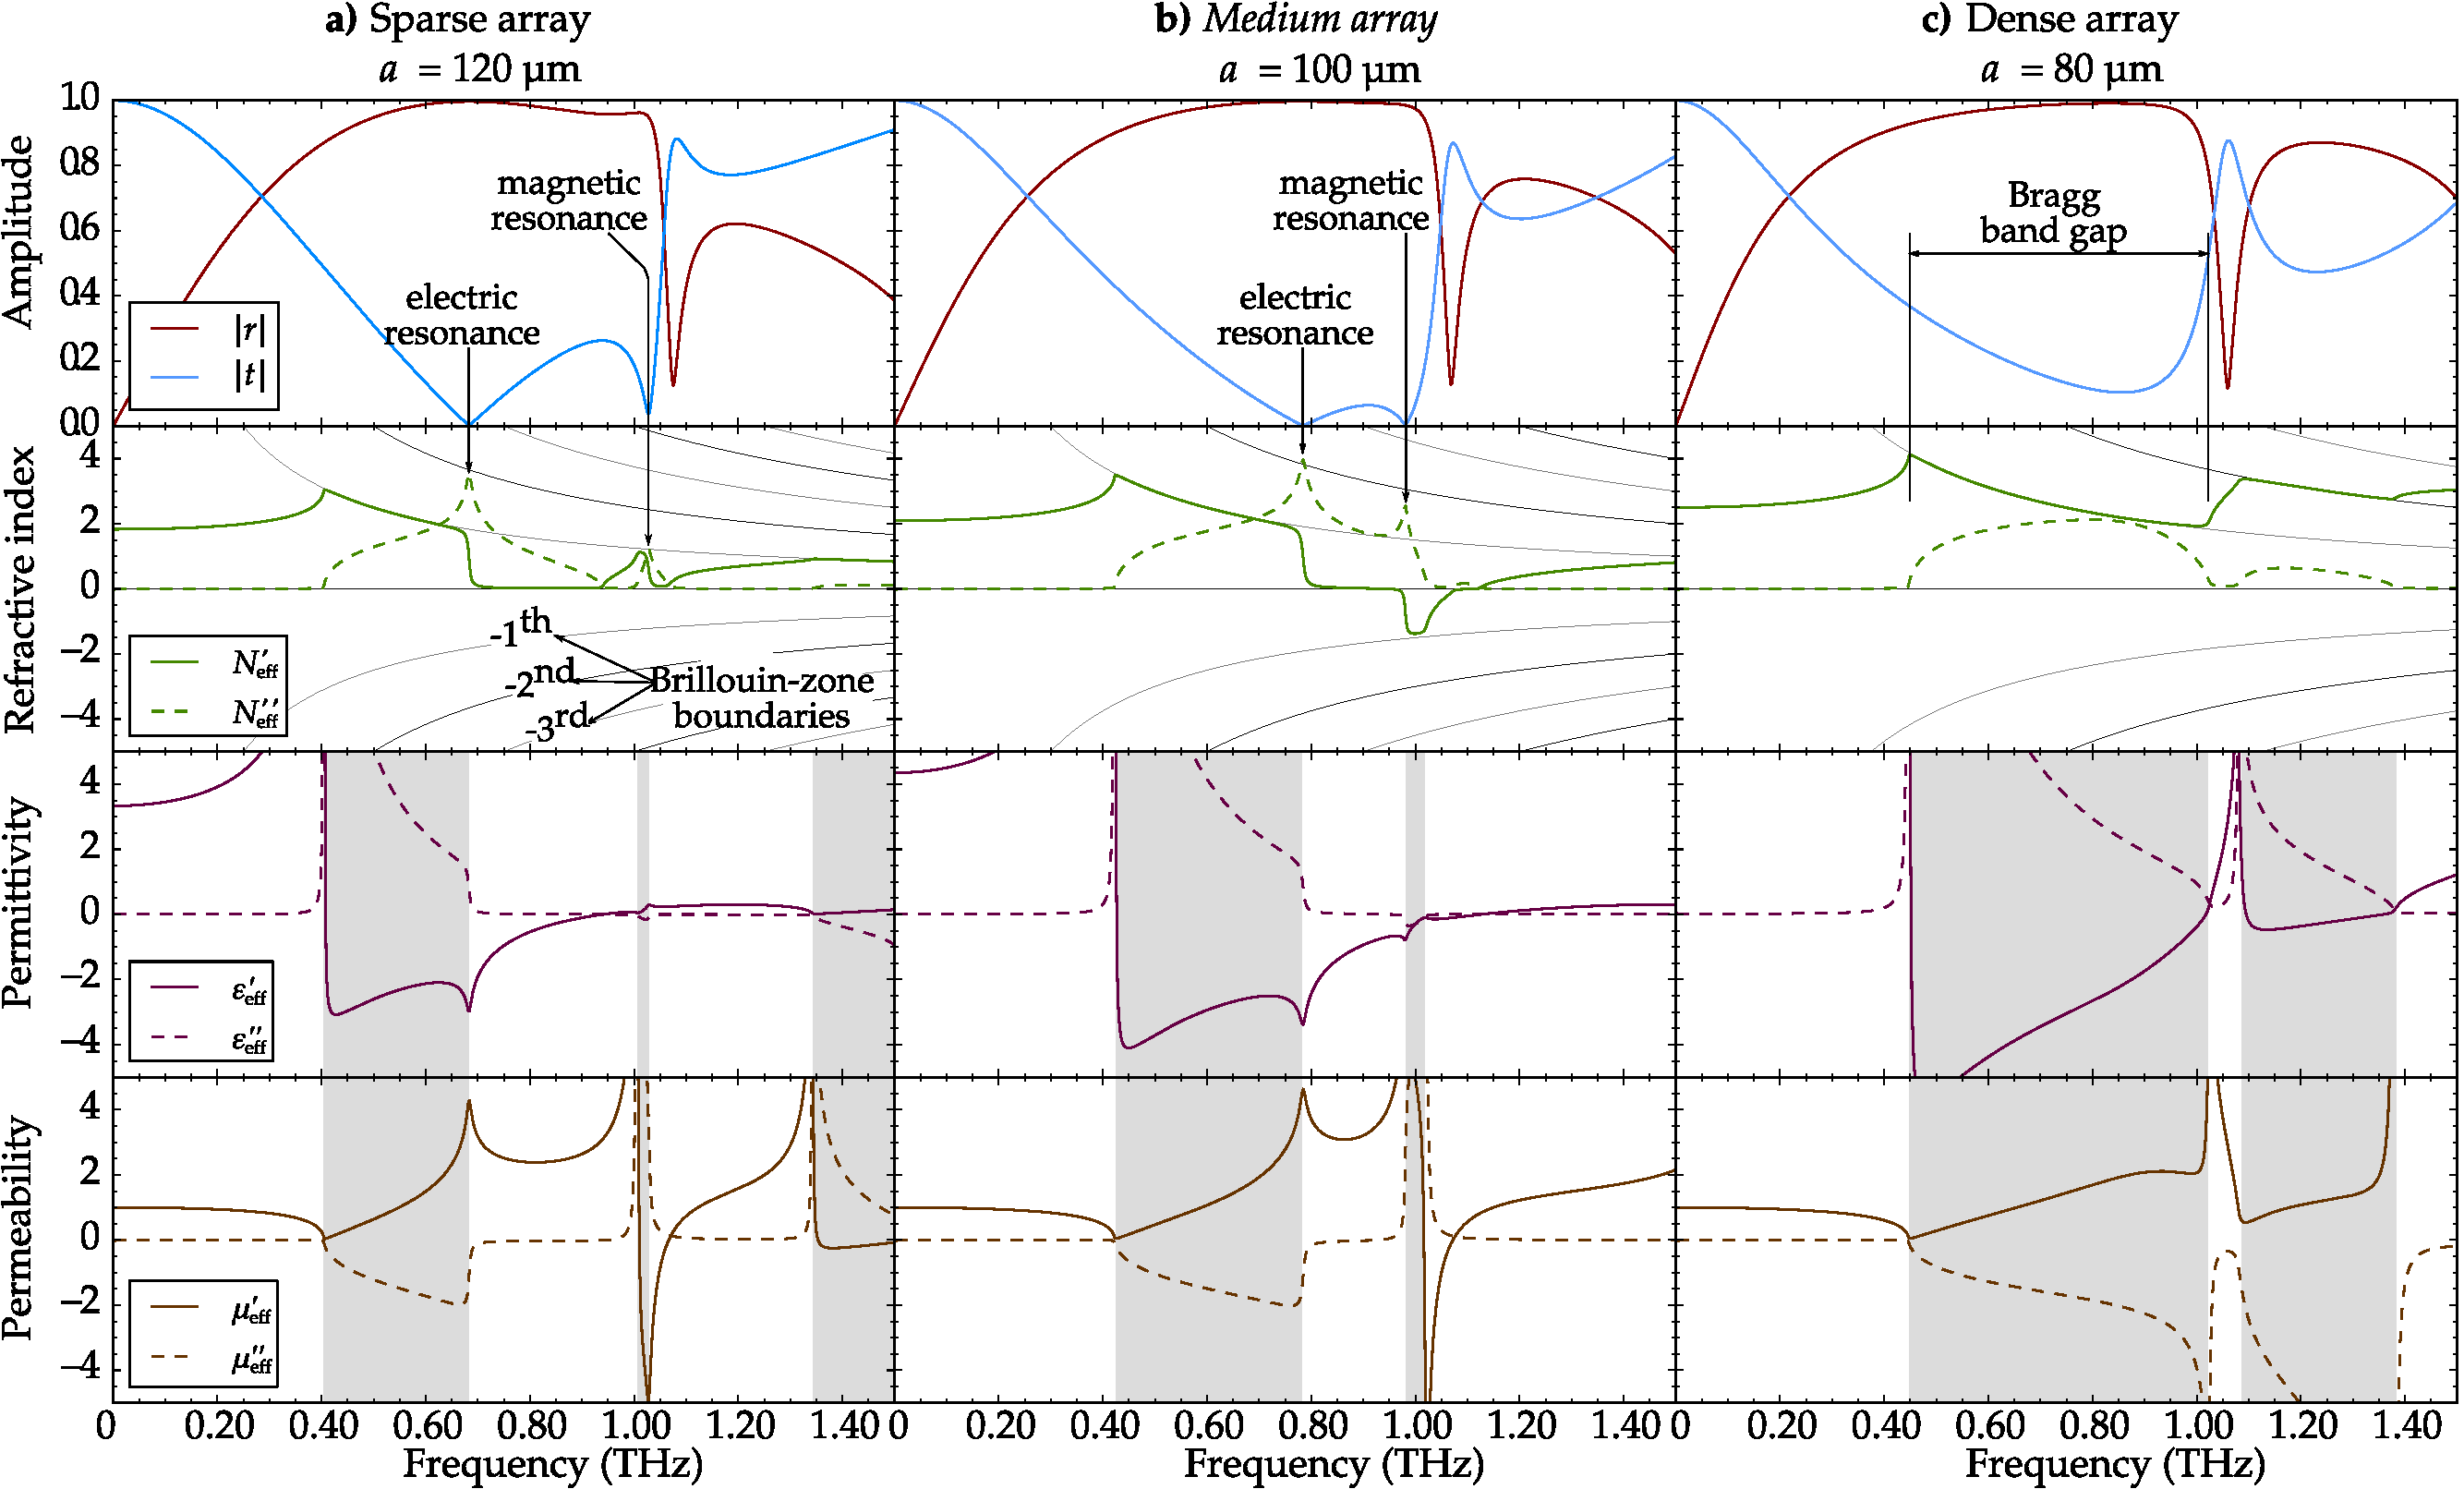
\includegraphics[width=10cm]{img/ERods_eps100_triple_a150a100a080_FDTD.pdf} \end{figure} \clearpage
%  \begin{figure} \caption{img/ERods\_forSeefeld\_sparserN\_denserN\_DrawnBands.pdf}  \centering 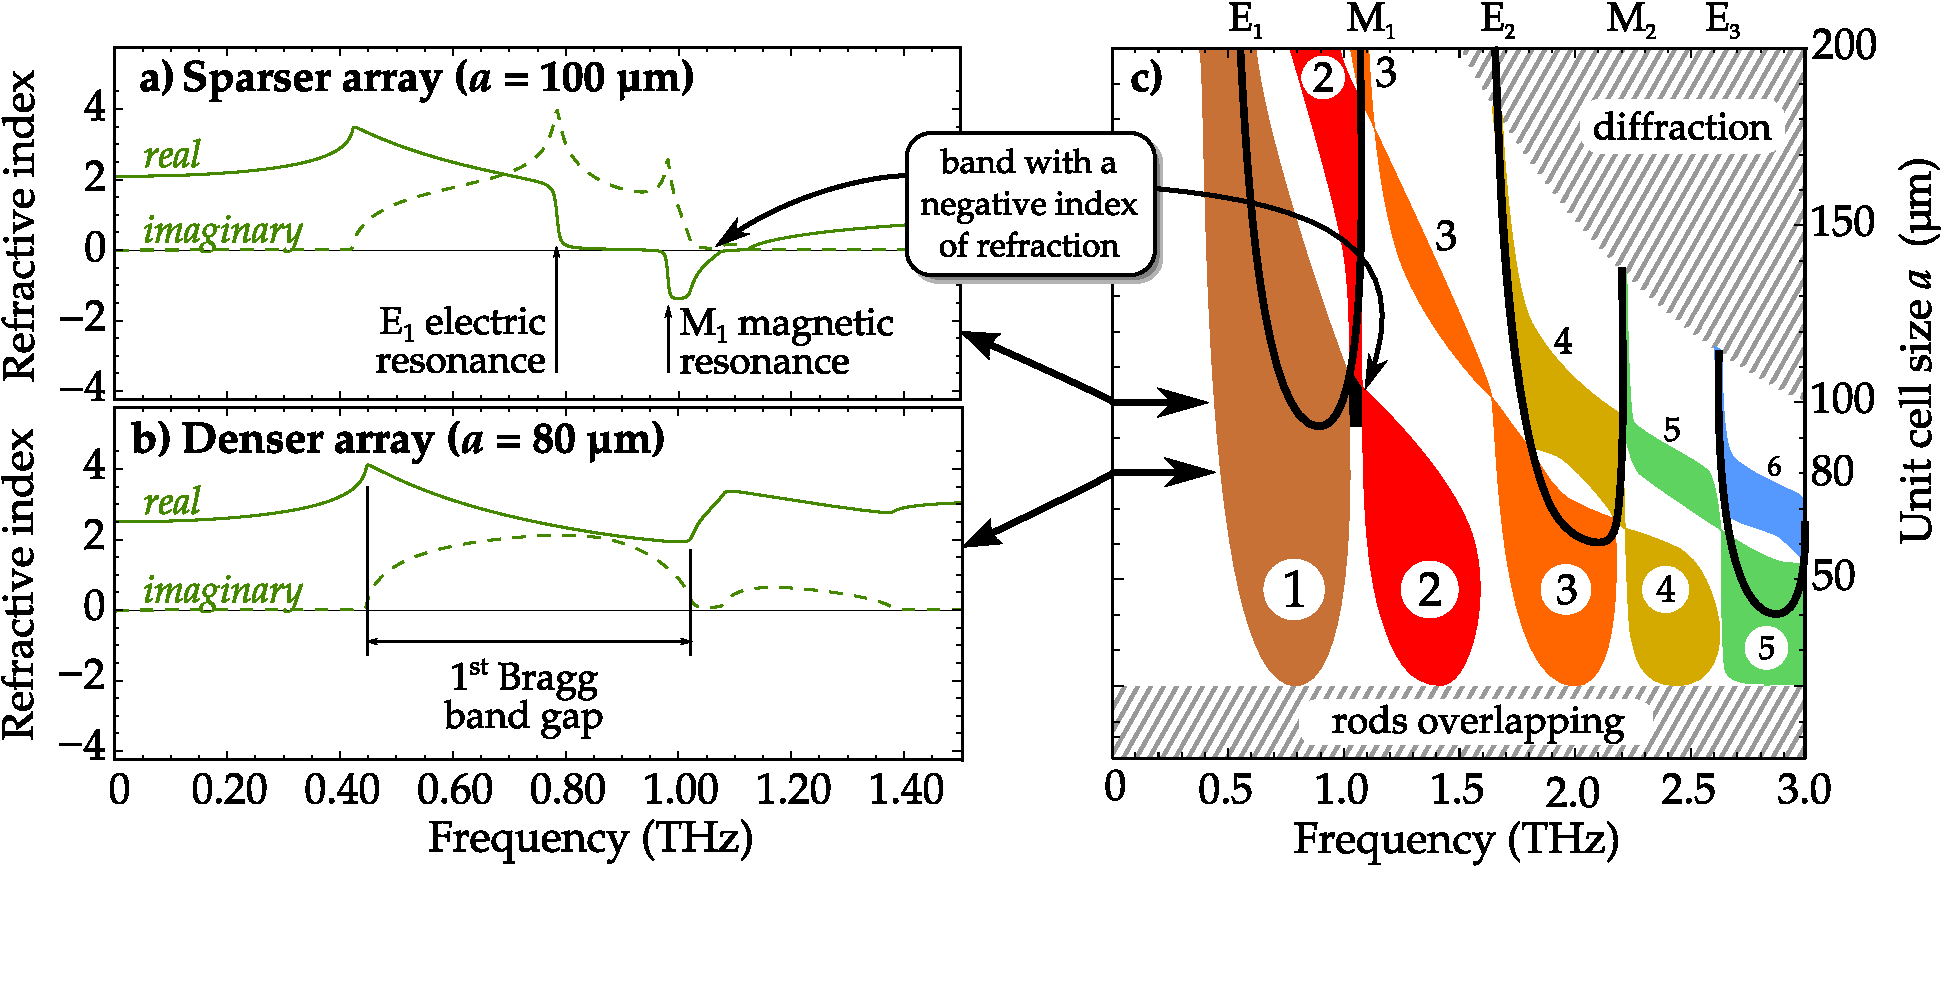
\includegraphics[width=10cm]{img/ERods_forSeefeld_sparserN_denserN_DrawnBands.pdf} \end{figure} \clearpage

\begin{figure} \caption{img/ERods\_sketch\_recordedline.pdf}  \centering  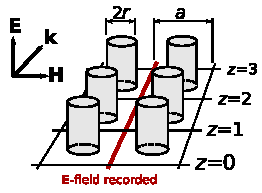
\includegraphics[width=10cm]{img/ERods_sketch_recordedline.pdf} \end{figure} \clearpage
\begin{figure} \caption{img/ERods\_eps100\_R10u5\_FXplot.pdf}  \centering 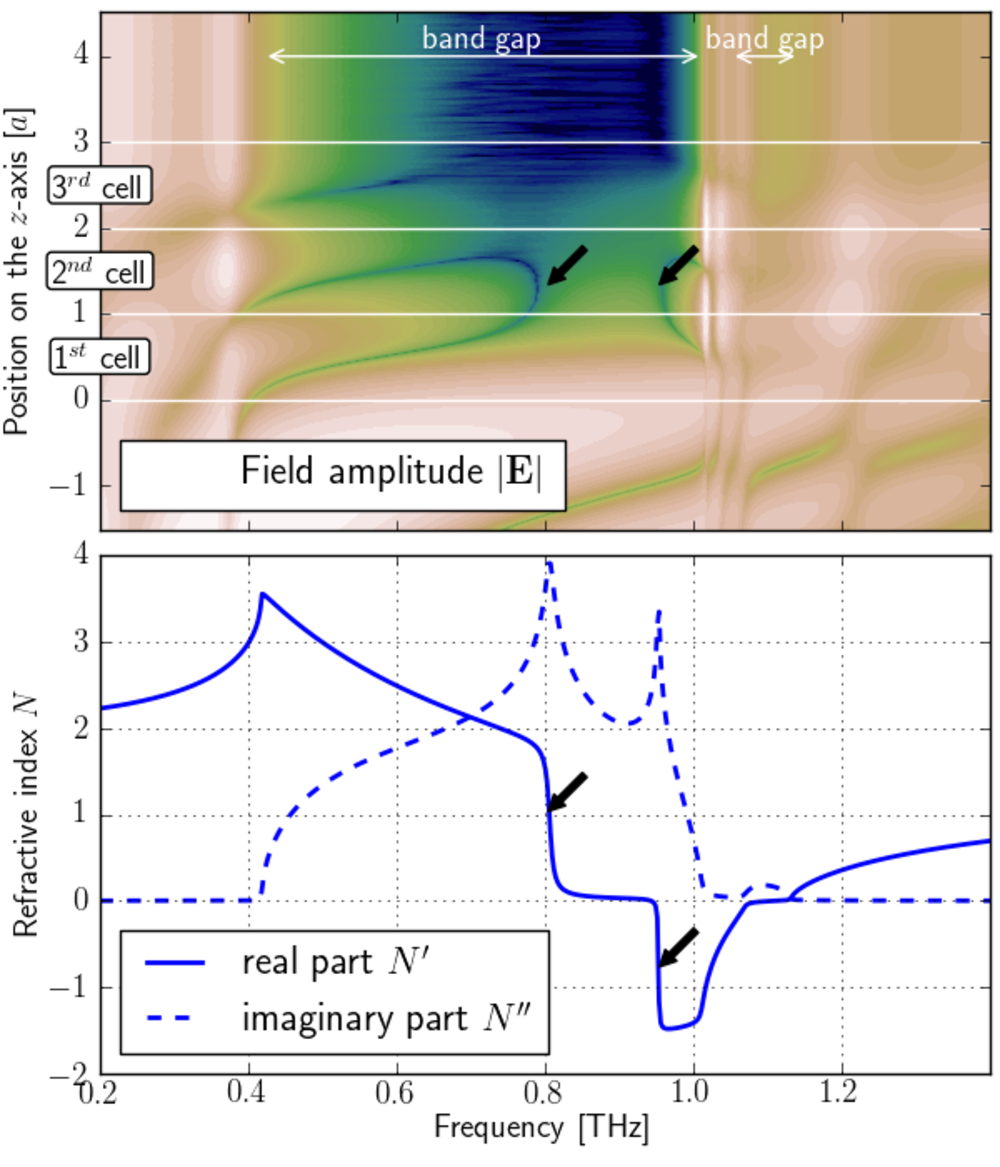
\includegraphics[width=10cm]{img/ERods_eps100_R10u5_FXplot.pdf} \end{figure} \clearpage

\section{Metallic screen with a slit} % references to ->

\section{A fishnet - metallic screen with holes} % references to ->
%{{{
\begin{figure} \caption{img/fishnet.pdf}  \centering \includegraphics[width=10cm]{img/fishnet.pdf} \end{figure} \clearpage
%}}}

\section{Other structures} % plasmonic spheres (note: resonance width determined by gamma of the metal?)
\begin{figure} \caption{Modes in sphere-wire structure}  \centering \includegraphics[width=10cm]{img/new/modes_Mag_and_El.pdf} \end{figure} \clearpage
\subsection{} % references to ->
\subsection{} % references to ->
\subsection{} % references to ->
\subsection{} % references to ->
\subsection{} % references to ->
